\documentclass[a4paper,12pt]{article}
\usepackage[utf8]{inputenc}
\usepackage{amsmath, amssymb, amsthm}
\usepackage{geometry}
\geometry{a4paper, margin=20mm, top=25mm, bottom=25mm}
\usepackage{multicol}
\usepackage{enumitem}
\usepackage[T1]{fontenc}
\usepackage[serbian]{babel} % Podeseno za latinicu
\usepackage{mathtools,amsfonts}
\usepackage{hyperref}
\usepackage{titlesec}

\hypersetup{
    colorlinks=true,
    citecolor=black,
    filecolor=black,
    linkcolor=black,
    urlcolor=blue
}

% Podesavanje naslova sekcija
\titleformat{\section}{\normalfont\large\bfseries}{\thesection.}{0.5em}{}
\titleformat{\subsection}{\normalfont\normalsize\bfseries\itshape}{\thesubsection.}{0.5em}{}

% Matematicke okoline na latinici
\theoremstyle{plain}
\newtheorem{theorem}{Teorema}[section]
\newtheorem{lemma}[theorem]{Lema}
\newtheorem{corollary}[theorem]{Posledica}

\theoremstyle{definition}
\newtheorem{definition}{Definicija}[section]
\newtheorem{example}{Primer}[section]

\theoremstyle{remark}
\newtheorem*{remark}{Napomena}

% Definicija lokalnih matematickih funkcija standardnih za nase podrucje
\renewcommand{\tan}{\operatorname{tg}}
\newcommand{\coloneqq}{\mathrel{\mathop:}=}
\renewcommand{\cot}{\operatorname{ctg}}
\renewcommand{\arctan}{\operatorname{arctg}}
\newcommand{\arccot}{\operatorname{arcctg}}

\begin{document}

% Glavni naslov u stilu sa slike
\begin{center}
    \vspace*{5mm}
    {\large\bfseries Ispitna pitanja iz Analize 1 (Informatika)} \\
    \vspace{2mm}
    {\large\bfseries --- Odgovori na pitanja ---} \\
    \vspace{2mm}
    {\large\bfseries 2025/2026} \\
    \vspace{4mm}
    {\itshape Kosta Čolović} \\
    \vspace{2mm}
    {\small Poslednja izmena: \today}
\end{center}
\vspace{8mm}
\textit{Na kraju dokumenta se nalazi sadržaj, radi brže navigacije.}


\section{Princip matematičke indukcije}
\noindent Neka je $P(n)$ iskaz koji zavisi od prirodnog broja $n$. Ako važi
\[ P(1) \land (\forall n \in \mathbb{N})\; P(n) \implies P(n+1), \]
tada je iskaz $P(n)$ tačan za sve prirodne brojeve.

\section{Arhimedovo i Kantorovo svojstvo skupa \texorpdfstring{$\mathbb{R}$}{R}}
\subsection{Arhimedova aksioma} 
\noindent \textbf{(ARH)}
\[ (\forall a > 0)(\forall b)(\exists n \in \mathbb{N})\; n \cdot a > b \]
U prevodu, koliko god bio velik broj $b$, ako dovoljan broj puta saberemo $a$ sa samim sobom, u nekom trenutnku ćemo preskočiti $b$.
\begin{figure}[!h]
    \centering
    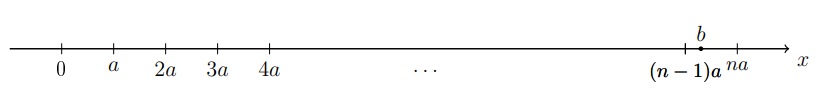
\includegraphics[width=1\textwidth]{slike/1-5.png}
\end{figure}
\subsection{Kantorova aksioma}
\begin{definition}
    Neka je dat niz nepraznih zatvorenih intervala $I_n = [a_n, b_n],\; n \in \mathbb{N}$. Ovaj niz nazivamo \textbf{nizom umetnutih intervala} ako za svako $n \in \mathbb{N}$ važi 
    $ I_{n+1} \subseteq I_n$.
\end{definition}
\noindent \textbf{(KAN)} Svaki niz zatvorenih umetnutih intervala ima neprazan presek, tj.
\[ \bigcap_{n \in \mathbb{N}} I_n \neq \emptyset \]

\section{Polje realnih brojeva}
\begin{definition}
    Uređena šestorka $(\mathbb{R}, +, \cdot, \leq, 0, 1)$ koja zadovoljava sledeće aksiome
    \begin{description}
        \item[(A1)] $(x + y) + z = x +(y + z)$\;\;(asocijativnost sabiranja)
        \item[(A2)] $x + 0 = 0 + x = x$\;\;(neutral za sabiranje)
        \item[(A3)] $(\forall x)(\exists y)\;x + y = y + x = 0$\;\;(postojanje inverznog elementa za sabiranje) 
        \item[(A4)] $x + y = y + x$\;\;(komutativnost sabiranja)
        \item[(A5)] $(x\cdot y) \cdot z = x \cdot (y \cdot z)$\;\; (asocijativnost množenja)
        \item[(A6)] $x \cdot 1 = 1 \cdot x = x$\;\; (element $1$ je neutral za množenje)  
        \item[(A7)] $x \cdot (y + z) = x\cdot y + x\cdot z,\; (x+y)\cdot z = x\cdot z + y\cdot z$\;\;(distributivnost mn. u odnosu na sab.)
        \item[(A8)] $x \cdot y = y \cdot x$\;\;(komutativnost množenja)
        \item[(A9)] $(\forall x \neq 0)(\exists y)\;x \cdot y = y \cdot x = 1$\;\;(svaki element razl. od 0 ima inverz u odnosu na množenje)
        \item[(A10)] $0 \neq 1$\;\;(netrivijalnost)
        \item[(A11)] $x \leq x$
        \item[(A12)] $x \leq y \land y \leq z \implies x \leq z$
        \item[(A13)] $x \leq y \land y \leq x \implies x = y$
        \item[(A14)] $x \leq y \lor y \leq x$
        \item[(A15)] $x \leq y \implies x + z \leq y + z$
        \item[(A16)] $x \geq 0 \land y \geq 0 \implies x \cdot y \geq 0$
        \item[(ARH)]
        \item[(KAN)]  
    \end{description}
    naziva se \textbf{poljem realnih brojeva}.
\end{definition}
\begin{theorem}
    \textbf{(Bernulijeva nejednakost):} Za sve $n \in \mathbb{N}$ i $\alpha \in \mathbb{R},\; \alpha > -1$ važi
    \[ (1 + \alpha)^n \geq 1 + n\alpha \]
    Dokaz indukcijom po $n$.
\end{theorem}

\section{Supremum i infimum skupa. Aksioma supremuma. Broj \texorpdfstring{$e$}{e}}
\subsection{Supremum i infimum skupa}
\begin{definition}
    Neka je $S \subseteq \mathbb{R}$. Kažemo da je $x \in \mathbb{R}$ \textbf{majoranta (gornje ograničenje)} skupa $S$ ako važi $(\forall s \in S)\; s \leq x$. Skup gornjih ograničenja označavamo sa $S^\leq$. Kažemo da je skup $S$ ograničen odozgo ako važi $x \in S^\leq$ i $x \in S$. Analogno se definiše i minoranta.
\end{definition}
\begin{definition}
    \textbf{Supremum} $\sup S$ skupa $S$ je, ako postoji, najmanje gornje ogr. skupa $S$.
\end{definition}
\begin{definition}
    \textbf{Infimum} $\inf S$ skupa $S$ je, ako postoji, najveće donje ograničenje skupa $S$.
\end{definition}
\subsection{Aksioma supremuma}
\begin{description}
    \item[(SUP)] Svaki neprazan, odozgo ograničen podskup ima supremum.
\end{description}
\begin{theorem}
    Svaki neprazan i odozgo ograničen podskup skupa realnih brojeva ima supremum.
\end{theorem}
\begin{proof} Neka je $S \subseteq \mathbb{R}$ neprazan i odozgo ograničen skup. Označimo
sa $s$ element skupa $S$, za koji znamo da postoji, a sa $x$ jedno njegovo gornje ograničenje.
\begin{itemize}
    \item Na osnovu Arhimedove aksiome, postoji prirodan broj $k$, takav da je $s + \frac{k}{2^2}$ gornje ograničenje skupa $S$. 
    \item Posmatrajmo niz brojeva $a_n$ i $b_n$ definisan na sledeći način: $a_1 := s,
    \; b_1 := x$. Svaki sledeći element se definiše kao $b_n := s + \frac{m_n}{2^n}$, gde je $m_n$ najmanji
    prirodan broj $k$ za koji važi da je $s + \frac{k}{2^n}$ gornje ograničenje skupa $S$; $a_n := s + \frac{m_n-1}{2^n}$.
    Pošto je $b_n$ gornje ograničenje skupa $S$, po definiciji važi da je $s' \leq b_n$, za svako $s' \in S$.
    Kako je $m_n$ najmanji broj $k \in \mathbb{N}$ za koji je $s + \frac{k}{2^n}$ gornje ograničenje skupa $S$, to znači da
    $m_n - 1$ nije gornje ograničenje skupa $S$. Dakle, ako $a_n = s + \frac{m_n-1}{2^n}$ nije gornje ograničenje, 
    to po definiciji znači da postoji bar jedan element $s^* \in S$ koji je strogo veći od njega. Odavde dobijamo da važi 
    $a_n < s^* \leq b_n$, odakle sledi $s^* \in [a_n, b_n] \cap S$. Dakle, $[a_n, b_n] \cap S \neq \emptyset$.
    \item Kako je $[a_{n+1}, b_{n+1}] \subseteq [a_n, b_n]$ (jer $a_n \leq a_{n+1}$ i $b_n \geq b_{n+1}$), za svako $n \in \mathbb{N}$, sledi da je $[a_n, b_n],\;n\in \mathbb{N}$ niz 
    umetnutih intervala. Prema kantorovoj teoremi, važi $\bigcap_{n \in \mathbb{N}} [a_n, b_n] \neq \emptyset$. 
    \item Pretpostavimo da postoje različiti elementi $x$ i $y$ td.
    $x, y \in \bigcap_{n \in \mathbb{N}} [a_n, b_n]$. Neka je, bez umanjenja opštosti, $x < y$. Kako $x$ i $y$ pripadaju svakom
    segmentu $[a_n, b_n]$, važiće \[0 < y-x < b_n - a_n = \left(s + \frac{m_n}{2^n}\right) - \left(s + \frac{m_n - 1}{2^n}\right) = \frac{1}{2^n},\]
    za svako $n \in \mathbb{N}$. Međutim, na osnovu Arhimedove aksiome, postoji dovoljno veliko $n \in \mathbb{N}$ td. $\frac{1}{2^n} < y - x$. Dobijamo 
    $y - x < \frac{1}{2^n} < y - x \implies y - x < y - x$, što je kontradikcija. Dakle postoji jedinstveno $s_0 \in \bigcap_{n \in \mathbb{N}} [a_n, b_n]$.
    \item Pretpostavimo da $s_0$ nije gornje ograničenje skupa $S$. To znači da postoji $s \in S$, td. $s - s_0 > 0$. Sa druge strane, znamo da za svako $n \in \mathbb{N}$
    važi $s \leq b_n$ (jer je $b_n$ gornje ograničenje skupa $S$), kao i da $s_0 \in [a_n, b_n]$, što znači da je $s_0 \leq b_n$, a rastojanje između njih ne može biti veće od
    dužine samog segmenta: \[ b_n - s_0 \leq b_n - a_n = \frac{1}{2^n} \] Prema Arhimedovoj aksiomi, pošto je $s-s_0$ fiksiran pozitivan broj, možemo izabrati dovoljno veliko $n \in \mathbb{N}$ td.
    dužina segmenta postane strogo manja od tog broja: \[ \frac{1}{2^n} < s - s_0 \]
    Dakle, važi: \[ b_n - s_0 \leq \frac{1}{2^n} < s- s_0 \implies b_n - s_0 < s - s_0 \implies b_n < s \]
    Dobili smo $b_n < s$, što je direktna kontradikcija sa činjenicom da je $b_n$ gornje ograničenje skupa $S$, dakle $s_0$ jeste gornje ograničenje skupa $S$.

    Da bismo dokazali da je $s_0$ najmanje gornje ograničenje, iskoristićemo standardnu $\varepsilon$-karakterizaciju supremuma: $$\forall \varepsilon > 0, \quad \exists s^* \in S \quad \text{tako da je} \quad s^* > s_0 - \varepsilon$$Uzmimo proizvoljno $\varepsilon > 0$. Ponovo se pozivamo na Arhimedovu aksiomu i biramo dovoljno veliko $n \in \mathbb{N}$ tako da važi:$$\frac{1}{2^n} < \varepsilon$$Pošto $s_0 \in [a_n, b_n]$, rastojanje između $s_0$ i leve ivice $a_n$ je takođe manje ili jednako od ukupne dužine segmenta:$$s_0 - a_n \leq b_n - a_n = \frac{1}{2^n} < \varepsilon$$Iz $s_0 - a_n < \varepsilon$ direktno sledi:$$a_n > s_0 - \varepsilon$$Sada se vraćamo na definiciju niza $a_n$. Znamo da $a_n = s + \frac{m_n - 1}{2^n}$ nije gornje ograničenje skupa $S$ (jer je $m_n$ izabran kao najmanji indeks za koji gornje ograničenje važi).Pošto $a_n$ nije gornje ograničenje, po definiciji postoji neki element $s^* \in S$ koji je strogo veći od njega:$$\exists s^* \in S, \quad s^* > a_n$$Spajanjem ove dve ključne nejednakosti dobijamo:$$s^* > a_n > s_0 - \varepsilon \implies s^* > s_0 - \varepsilon$$
\end{itemize}
\end{proof}

\begin{theorem}
    Svaki neprazan i odozdo ograničen podskup skupa realnih brojeva ima infimum.
\end{theorem}
\begin{proof}
    Analogno prethodnom dokazu.
\end{proof}
\subsection{Broj $e$}
\label{4-3}
\[ \bigg( 1 + \frac{1}{n} \bigg)^n = 1 + \sum_{n}^{k = 1}{{n} \choose {k}} \frac{1}{n^k} = 1 + {{n} \choose 1} \frac{1}{n} + \sum_{k = 2}^{n}\frac{n(n-1)\dots (n-k+1)}{k! \cdot n^k}\]
\[\leq 1 + 1 + \sum_{k = 2}^{n} \frac{1}{k(k-1)} = 2 + \sum_{k = 2}^{n}\bigg(\frac{1}{k-1} - \frac{1}{k}\bigg) = 2 + 1 - \frac{1}{n} < 3\]
Dakle, skup \[ E = \bigg\{ \bigg( 1 + \frac{1}{n} \bigg)^n \; \bigg|\; n \in \mathbb{N} \bigg\} \] je ograničen odozgo brojem 3 i neprazan jer $2 \in E$. Supremum ovog skupa (koji postoji zbog aksiome supremuma) je Ojlerov broj $e \approx 2.71828$. On je iracionalan i transcendentan.
 
\newpage
\section{Prošireni skup realnih brojeva}
\begin{definition}
    \[ \overline{\mathbb{R}} := \mathbb{R} \cup \{-\infty\} \cup \{+\infty\} \]
    \[ -\infty < x < +\infty, \; x \in \mathbb{R} \]
\end{definition}

\begin{description}
    \item[(1)] $x + (+ \infty) = + \infty, \; -\infty < x \leq +\infty$
    \item[(2)] $x + (- \infty) = -\infty, \; -\infty \leq x < +\infty$
    \item[(3)] $\frac{x}{+\infty} = \frac{x}{-\infty},\; x \in \mathbb{R}$
    \item[(4)] $x \cdot (\pm \infty) = \pm \infty,\; 0 < x \leq +\infty$  
    \item[(5)] $x \cdot (\pm \infty) = \mp \infty, \; -\infty \leq x < 0$
\end{description}

\section{Definicija granične vrednosti niza i primeri}
\begin{definition}
    Kažemo da niz realnih brojeva $(x_n)$ ima limes $x_\infty$ ako važi:
    \[ (\forall \varepsilon > 0)(\exists n_0 \in \mathbb{N})(\forall n \in \mathbb{N}) \; n \geq n_0 \implies |x_n - x_\infty| < \varepsilon \]
    Tada kažemo da on konvergira i pišemo $\lim_{x \to +\infty} x_n$. U suprotnom, kažemo da divergira.
\end{definition}
\begin{definition}
    Kažemo da niz realnih brojeva $x_n$ ima limes $+\infty$ ako važi:
    \[ (\forall M \in \mathbb{R})(\exists n_0 \in \mathbb{N})(\forall n \in \mathbb{N}) \; n \geq n_0 \implies x_n > M \]
    Analogno, kažemo da niz realnih brojeva $x_n$ ima limes $-\infty$ ako važi:
    \[ (\forall M \in \mathbb{R})(\exists n_0 \in \mathbb{N})(\forall n \in \mathbb{N}) \; n \geq n_0 \implies x_n < M \]
\end{definition}
\section{Svojstva konvergentnih nizova (algebarske operacije)}
\begin{definition}
    Kažemo da je niz $(x_n)$ ograničen ako postoji broj $M \in \mathbb{R}$ takav da važi $|x_n| \leq M$ za sve $n \in \mathbb{N}$. Broj $M$ nazivamo ograničenjem niza $(x_n)$.
\end{definition}
\begin{theorem}
    Niz $(x_n)$ konvergira $\implies$ niz $(x_n)$ je ograničen.
\end{theorem}
\begin{proof}
    Neka je $(x_n)$ konvergentan i neka je njegov limes $x_\infty \in \mathbb{R}$. Za $\varepsilon = \frac{1}{2}$ postojaće $n_0 \in \mathbb{N}$ td. $|x_n - x_\infty| < \frac{1}{2}$ za sve $n \geq n_0$. 
    Dakle, $x_{n_0}, x_{n_0 + 1}, x_{n_0 + 2}, \ldots \in (x_\infty - \frac{1}{2}, x_\infty + \frac{1}{2})$.  Neka je
    \[ M_1 = \max \bigg\{ \bigg|x_\infty - \frac{1}{2}\bigg|, \bigg|x_\infty + \frac{1}{2}\bigg|  \bigg\}. \]
    Tada je $|x_\infty| \leq M$ za sve $n \geq n_0$. Definišemo 
    \[ M = \max \{ |x_1|, |x_2|, \ldots, |x_{n_0-1}|, M_1 \}. \]
    Ovo je jedno ograničenje niza $(x_n)$.
\end{proof}
\newpage
\begin{lemma}
    Neka je $(x_n)$ niz realnih brojeva. Tada je $\lim_{n \to +\infty}x_n = 0 \iff \lim_{x \to +\infty}|x_n| = 0$.
\end{lemma}
\begin{proof}
    \[
        \begin{aligned}
            &\lim_{x \to +\infty} x_n = 0 \\
            \iff &(\forall \varepsilon > 0)(\exists n_0 \in \mathbb{N})(\forall n \in \mathbb{N}) \; n \geq n_0 \implies |x_n - 0| < \varepsilon \\
            \iff &(\forall \varepsilon > 0)(\exists n_0 \in \mathbb{N})(\forall n \in \mathbb{N}) \; n \geq n_0 \implies |x_n| < \varepsilon \\
            \iff &(\forall \varepsilon > 0)(\exists n_0 \in \mathbb{N})(\forall n \in \mathbb{N}) \; n \geq n_0 \implies ||x_n||< \varepsilon \\
            \iff &(\forall \varepsilon > 0)(\exists n_0 \in \mathbb{N})(\forall n \in \mathbb{N}) \; n \geq n_0 \implies ||x_n| - 0| < \varepsilon \\
            \iff &\lim_{n \to +\infty} |x_n| = 0
        \end{aligned}
    \]
\end{proof}

\begin{theorem}
    Neka su $(x_n)_{n \in \mathbb{N}}$ i $(y_n)_{n \in \mathbb{N}}$ konvergentni 
    nizovi. Tada važi sledeće:
    \begin{enumerate}
        \item \textbf{(Linearnost limesa)} Niz $(\lambda x_n + \mu y_n)_{n \in \mathbb{N}}$ je konvergentan za sve realne br. $\lambda$ i $\mu$ i važi
        \[ \lim_{n \to +\infty}(\lambda x_n + \mu y_n) = \lambda \lim_{n \to +\infty}x_n + \mu \lim_{n \to +\infty}y_n \]
        \item Niz $(x_n \cdot y_n)_{n \in \mathbb{N}}$ je konvergentan i važi
        \[ \lim_{n \to +\infty}(x_n \cdot y_n) = \lim_{n \to +\infty} x_n \cdot \lim_{n \to + \infty}y_n \]
        \item Ako su članovi niza $(y_n)_{n \in \mathbb{N}}$ različiti od nule i ako je $\displaystyle \lim_{n \to +\infty} y_n \neq 0$, tada je niz $\displaystyle \bigg(\frac{x_n}{y_n}\bigg)_{n \in \mathbb{N}}$ konvergentan i važi
        \[ \lim_{n \to +\infty}\frac{x_n}{y_n}= \frac{\displaystyle \lim_{n \to +\infty} x_n}{\displaystyle \lim_{n \to +\infty} y_n} \]
    \end{enumerate}
\end{theorem}
\begin{proof}
    \begin{enumerate}
        \item Uzmimo proizvoljno $\varepsilon > 0$ i pretpostavimo da $\mu \neq 0 \land \lambda \neq 0$. Na osnovu konvergencije zaključujemo da postoje $n_1, n_2$, td. za $n\geq n_1$ i $n \geq n_2$ respektivno
        važe sledeće nejednakosti:
        \[ |x_n - x_\infty| < \frac{\varepsilon}{2|\lambda|}, \;\;\; |y_n - y_\infty| < \frac{\varepsilon}{2|\mu|}.  \]
        Neka je $n_0 = \max\{n_1, n_2\}$. Tada za sve $n \geq n_0$ važi
        \[
            \begin{aligned}
                |\lambda x_n + \mu y_n - (\lambda x_\infty + \mu y_\infty)| &\leq |\lambda x_n - \lambda x_\infty| + |\mu y_n - \mu y_\infty| = \\
                &= |\lambda|\cdot |x_n - x_\infty| + |\mu| \cdot |y_n - y_\infty| < \\
                & < |\lambda| \cdot \frac{\varepsilon}{2 |\lambda|} + |\mu| \cdot \frac{\varepsilon}{2|\mu|} = \varepsilon
            \end{aligned}
        \]  
        Slučajevi gde su oba ili jedan od $\lambda, \mu$ jednak nula se lako dokazuju. Dakle, zaključujemo da je niz konvergentan i da je njegova granična vrednost $\lambda x_\infty + \mu y_\infty$.
        
        \item Neka je $\lim_{n \to +\infty} x_n = x_\infty$ i $\lim_{n \to +\infty} y_n = y_\infty$. Kako je svaki konvergentan niz ograničen, to postoji konstanta $M > 0$ takva da je $|x_n| \leq M$ za sve $n \in \mathbb{N}$. Takođe, možemo pretpostaviti da je $|y_\infty| < M$ (ili jednostavno uzeti dovoljno veliko $M$).
        
        Uočimo transformaciju:
        \[
            |x_n y_n - x_\infty y_\infty| = |x_n y_n - x_n y_\infty + x_n y_\infty - x_\infty y_\infty| \leq |x_n| \cdot |y_n - y_\infty| + |y_\infty| \cdot |x_n - x_\infty|
        \]
        Fiksirajmo proizvoljno $\varepsilon > 0$. Na osnovu konvergencije nizova, postoje $n_1, n_2 \in \mathbb{N}$ takvi da:
        \[
            \text{za } n \geq n_1 \implies |y_n - y_\infty| < \frac{\varepsilon}{2M}, \;\;\; \text{za } n \geq n_2 \implies |x_n - x_\infty| < \frac{\varepsilon}{2M}.
        \]
        Neka je $n_0 = \max\{n_1, n_2\}$. Tada za sve $n \geq n_0$ važi:
        \[
            |x_n y_n - x_\infty y_\infty| \leq M \cdot |y_n - y_\infty| + M \cdot |x_n - x_\infty| < M \cdot \frac{\varepsilon}{2M} + M \cdot \frac{\varepsilon}{2M} = \varepsilon.
        \]
        Ovim je dokazano da je $\lim_{n \to +\infty} (x_n \cdot y_n) = x_\infty \cdot y_\infty$.

        \item Najpre dokažimo pomoćno tvrđenje da je $\lim_{n \to +\infty} \frac{1}{y_n} = \frac{1}{y_\infty}$. 
        
        Kako je $y_ \infty \neq 0$, to je $|y_\infty| > 0$. Iz definicije konvergencije, za $\varepsilon_0 = \frac{|y_\infty|}{2} > 0$ postoji $n_1 \in \mathbb{N}$ takvo da za sve $n \geq n_1$ važi $|y_n - y_\infty| < \frac{|y_\infty|}{2}$. Koristeći nejednakost trougla, imamo:
        \[
            |y_n| = |y_\infty - (y_\infty - y_n)| \geq |y_\infty| - |y_n - y_\infty| > |y_\infty| - \frac{|y_\infty|}{2} = \frac{|y_\infty|}{2}.
        \]
        Dakle, za $n \geq n_1$ važi $\frac{1}{|y_n|} < \frac{2}{|y_\infty|}$.
        
        Uzmimo sada proizvoljno $\varepsilon > 0$. Postoji $n_2 \in \mathbb{N}$ tako da za sve $n \geq n_2$ važi $|y_n - y_\infty| < \frac{\varepsilon \cdot |y_\infty|^2}{2}$.
        
        Neka je $n_0 = \max\{n_1, n_2\}$. Tada za sve $n \geq n_0$ važi:
        \[
            \left| \frac{1}{y_n} - \frac{1}{y_\infty} \right| = \frac{|y_\infty - y_n|}{|y_n| \cdot |y_\infty|} < \frac{2}{|y_\infty|^2} \cdot |y_n - y_\infty| < \frac{2}{|y_\infty|^2} \cdot \frac{\varepsilon \cdot |y_\infty|^2}{2} = \varepsilon.
        \]
        Dakle, $\lim_{n \to +\infty} \frac{1}{y_n} = \frac{1}{y_\infty}$.
        
        Konačno, primenom već dokazane tačke 2 na nizove $(x_n)$ i $(\frac{1}{y_n})$ dobijamo:
        \[
            \lim_{n \to +\infty} \frac{x_n}{y_n} = \lim_{n \to +\infty} \left( x_n \cdot \frac{1}{y_n} \right) = \lim_{n \to +\infty} x_n \cdot \lim_{n \to +\infty} \frac{1}{y_n} = x_\infty \cdot \frac{1}{y_\infty} = \frac{x_\infty}{y_\infty}.
        \]
    \end{enumerate}
\end{proof}

\begin{theorem}
    Neka su $(x_n)$ i $(y_n)$ konvergentni nizovi takvi da za sve $n \in \mathbb{N}$ važi $\displaystyle x_n \leq y_n$. Tada važi
    \[ \lim_{n \to +\infty} x_n \leq \lim_{n \to +\infty} y_n. \]
\end{theorem}
\begin{proof}
Pretpostavimo suprotno: $\displaystyle x_\infty := \lim_{n \to +\infty} x_n > \lim_{n \to +\infty} y _n =: y_\infty$. Neka je $\varepsilon = \frac{x_\infty - y_\infty}{3}$.
Neka su $n_1, n_2 \in \mathbb{N}$ td. $|x_n - x_\infty| < \varepsilon, \; |y_n - y_\infty| < \varepsilon$ za $n \geq n_1$ i $n \geq n_2$ respektivno. Neka je sada $n_0 = \max\{n_1, n_2\}$.
Dakle, za svako $n > n_0$ važi
\[ x_\infty - \varepsilon < x_n < x_\infty + \varepsilon, \; \;\;y_\infty - \varepsilon < y_n < y_\infty + \varepsilon \]
Odavde dolazimo do nejednakosti
\[ y_n < y_\infty + \varepsilon < x_\infty + \varepsilon < x_n, \]
koja je u kontradikciji sa pretpostavkom.
\end{proof}

\section{Teorema o tri limesa za nizove}
\begin{theorem}
    Neka su dati nizovi $(a_n), (b_n), (c_n)$ td. $a_n \leq b_n \leq c_n, \forall n \in \mathbb{N}$. Ako je \linebreak$\displaystyle \lim_{n \to +\infty} a_n = \lim_{n \to +\infty} c_n = d_\infty$, tada je i $\displaystyle \lim_{n \to +\infty} b_n = d_\infty$.
\end{theorem}
\begin{proof}
    Uzmimo proizvoljno $\varepsilon > 0$. Iz konvergencije nizova sledi da postoje $n_1, n_2 \in \mathbb{N}$ td. 
    \[ |a_n - d_\infty| < \varepsilon, \; \forall n \geq n_1 \land  |c_n - d_\infty| < \varepsilon , \; \forall n \geq n_2\]
    Tada za sve $n > \max\{n_1, n_2\}$ važi $d_\infty - \varepsilon < a_n$ i $d_\infty + \varepsilon > c_n$, odakle dobijamo
    \[ d_\infty - \varepsilon < a_n \leq b_n \leq c_n < d_\infty + \varepsilon \]
\end{proof}

\begin{theorem}
    Ako je $\lim_{n \to +\infty} x_n = 0$ i $(y_n)$ ograničen, tada važi
    \[ \lim_{n \to +\infty}(x_n \cdot y_n) = 0 \]
\end{theorem}
\begin{proof}
    Dokaz se oslanja na Teoremu o tri limesa: Pošto je $y_n$ ograničen, postoji neki realan broj $M > 0$ takav da je $|y_n| \le M$ za svako $n$.Ako pomnožimo tu nejednakost sa $|x_n|$, dobijamo:$$0 \le |x_n \cdot y_n| \le M \cdot |x_n|$$Kada pustimo da $n \to +\infty$, desna strana $M \cdot |x_n|$ teži nuli (jer $x_n \to 0$). Pošto je naš niz "uklešten" između nule i nečega što teži nuli, i on sam mora težiti nuli.
\end{proof}
\section{Štolcova teorema i posledice}
\begin{theorem}
    \textbf{(Štolc)} Ako je $(y_n)$ rastući i $\displaystyle \lim_{n \to + \infty} y_n = +\infty$. Tada važi:
    \[ \text{postoji } \lim_{n \to +\infty} \frac{x_{n+1} - x_n}{y_{n+1} - y_n} \in \overline{\mathbb{R}} \implies \lim_{n \to +\infty} \frac{x_n}{y_n} = \lim_{n \to +\infty} \frac{x_{n+1} - x_n}{y_{n+1} - y_n}\]
\end{theorem}
\begin{proof}
Ideja dokaza je da se $x_{n+1} - x_n$ ograniči odozdo i odozgo konstantom pomnoženom sa $y_{n+1} - y_n$, pa da se nejednakosti sumiraju po određenom skupu indeksa.

Prvo dokazujemo slučaj kada je limes konačan.

Označimo sa $L = \lim_{n \to +\infty} \frac{x_{n+1}-x_n}{y_{n+1}-y_n} \in \mathbb{R}$ i neka je $\varepsilon > 0$ proizvoljno. Postojaće $n_1 \in \mathbb{N}$ takvo da je za sve $n \geq n_1$
$$ \left| \frac{x_{n+1}-x_n}{y_{n+1}-y_n} - L \right| < \frac{\varepsilon}{3}. $$
Tada je
$$ L - \frac{\varepsilon}{3} < \frac{x_{n+1}-x_n}{y_{n+1}-y_n} < L + \frac{\varepsilon}{3} $$
za sve $n \geq n_1$ a kako je niz $(y_n)$ rastući onda je $y_{n+1} - y_n > 0$ pa time pomnožimo celu nejednakost
$$ \left(L - \frac{\varepsilon}{3}\right) (y_{n+1} - y_n) < x_{n+1} - x_n < \left(L + \frac{\varepsilon}{3}\right) (y_{n+1} - y_n). $$
Napišemo prethodnu nejednakost pomoću indeksa $i$ pa onda sumiramo te nejednakosti od $i = n_1$ do $i = n - 1$
$$ \sum_{i=n_1}^{n-1} \left(L - \frac{\varepsilon}{3}\right) (y_{i+1} - y_i) < \sum_{i=n_1}^{n-1} (x_{i+1} - x_i) < \sum_{i=n_1}^{n-1} \left(L + \frac{\varepsilon}{3}\right) (y_{i+1} - y_i). $$
Kako je $\sum_{i=n_1}^{n-1} (x_{i+1} - x_i) = x_n - x_{n_1}$ a ista formula važi kada sumiramo po $y$ dolazimo do nejednakosti
$$ \left(L - \frac{\varepsilon}{3}\right) (y_n - y_{n_1}) < x_n - x_{n_1} < \left(L + \frac{\varepsilon}{3}\right) (y_n - y_{n_1}) $$
koja važi za sve $n > n_1$. Sada podelimo sve sa pozitivnim brojem $y_n - y_{n_1}$ i dobijamo
$$ L - \frac{\varepsilon}{3} < \frac{x_n - x_{n_1}}{y_n - y_{n_1}} < L + \frac{\varepsilon}{3}, $$
odnosno
$$ \left| \frac{x_n - x_{n_1}}{y_n - y_{n_1}} - L \right| < \frac{\varepsilon}{3}. $$
Sada procenjujemo razliku količnika $x_n/y_n$ i vrednosti $L$
\begin{align*}
\left| \frac{x_n}{y_n} - L \right| &= \left| \frac{x_{n_1} - L y_{n_1}}{y_n} + \left(1 - \frac{y_{n_1}}{y_n}\right) \left( \frac{x_n - x_{n_1}}{y_n - y_{n_1}} - L \right) \right| \\
&\leq \left| \frac{x_{n_1} - L y_{n_1}}{y_n} \right| + \left| \left(1 - \frac{y_{n_1}}{y_n}\right) \left( \frac{x_n - x_{n_1}}{y_n - y_{n_1}} - L \right) \right| \\
&\leq \left| \frac{x_{n_1} - L y_{n_1}}{y_n} \right| + \frac{3}{2} \left| \frac{x_n - x_{n_1}}{y_n - y_{n_1}} - L \right| \\
&< \frac{\varepsilon}{2} + \frac{3}{2} \cdot \frac{\varepsilon}{3} = \varepsilon
\end{align*}
za sve $n > \max\{n_1, n_2, n_3\}$. Zaključujemo da je $\lim_{n \to +\infty} \frac{x_n}{y_n} = L$.

Sada ćemo prodiskutovati slučaj kada je $\lim_{n \to +\infty} \frac{x_{n+1}-x_n}{y_{n+1}-y_n} = +\infty$. Tada je $x_{n+1} - x_n$ veće od $17(y_{n+1}-y_n) > 0$ za dovoljno veliko $n$ pa će i niz $(x_n)$ biti rastući i težiti ka $+\infty$ pa onda posmatramo recipročnu vrednost $\lim_{n \to +\infty} \frac{y_{n+1}-y_n}{x_{n+1}-x_n} = 0$ i primenimo ono što smo dokazali. Tada će važiti $\lim_{n \to +\infty} \frac{y_n}{x_n} = 0$ a kako je ovo količnik pozitivnih veličina onda je $\lim_{n \to +\infty} \frac{x_n}{y_n} = +\infty$.

Ako je $\lim_{n \to +\infty} \frac{x_{n+1}-x_n}{y_{n+1}-y_n} = -\infty$ onda je $\lim_{n \to +\infty} \frac{(-x_{n+1})-(-x_n)}{y_{n+1}-y_n} = +\infty$ pa sad premenimo ono od malo pre i zaključujemo da će važiti $\lim_{n \to +\infty} \frac{(-x_n)}{y_n} = +\infty$ odnosno $\lim_{n \to +\infty} \frac{x_n}{y_n} = -\infty$.
\end{proof}
\textbf{Posledica 1.} (Košijeva teorema za nizove) Neka je $(a_n)$ konvergentan niz i neka je njegova granična vrednost $a_{\infty}$. Tada konvergira i niz aritmetičkih sredina
$$ A_n = \frac{a_1 + a_2 + \ldots + a_n}{n} $$
ka istoj graničnoj vrednosti, $\lim_{n \to +\infty} A_n = a_{\infty}$.

\begin{proof}
Dokaz sledi iz Štolcove teoreme kada je primenimo na nizove $x_n = a_1 + a_2 + \ldots + a_n$ i $y_n = n$.
\end{proof}

\textbf{Posledica 2.} Neka niz $(a_n)$ konvergira ka $a_{\infty}$. Tada konvergira i niz harmonijskih sredina
$$ H_n = \frac{n}{\frac{1}{a_1} + \frac{1}{a_2} + \ldots + \frac{1}{a_n}} $$
i važi $\lim_{n \to +\infty} H_n = a_{\infty}$.

\begin{proof}
Primenimo prethodnu posledicu na niz $\frac{1}{H_n}$.
\end{proof}

\textbf{Posledica 3.} Neka je $(a_n)$ konvergentan niz takav da je $a_n > 0$ za sve $n \in \mathbb{N}$. Niz geometrijskih sredina
$$ G_n = \sqrt[n]{a_1 a_2 \cdot \ldots \cdot a_n} $$
je takođe konvergentan niz i važi $\lim_{n \to +\infty} G_n = \lim_{n \to +\infty} a_n$.

\begin{proof}
Primenimo Štolcovu teoremu na niz $\ln G_n = \frac{\ln a_1 + \ln a_2 + \ldots + \ln a_n}{n}$.
\end{proof}

\section{Monotoni nizovi, egzistencija limesa}
\textbf{Teorema 28.} Neka je niz $(x_n)_{n \in \mathbb{N}}$ monoton. Tada je on konvergentan ako i samo ako je ograničen. Ako je niz neograničen onda je on određeno divergentan.
\begin{proof}
$\Longrightarrow$ : Ovaj smer je trivijalan jer znamo da je svaki konvergentan niz ograničen. Primetimo da nam za ovaj smer pretpostavka o monotonosti nije bila potrebna.

$\Longleftarrow$ : Neka je sada $(x_n)_{n \in \mathbb{N}}$ monoton i ograničen niz. Hoćemo da pokažemo da on konvergira. Pretpostavićemo da je niz rastući (ako je opadajući onda posmatramo niz $(-x_n)_{n \in \mathbb{N}}$ koji će biti rastući pa na njega primenimo dokazano). Skup
$$ X = \{x_n \mid n \in \mathbb{N}\} $$
je ograničen i neprazan pa na osnovu aksiome supremuma ima supremum. Označimo ga sa
$$ x_{\infty} = \sup X. $$
Pokazaćemo da je ovo $x_{\infty}$ granična vrednost našeg niza $(x_n)_{n \in \mathbb{N}}$.

Neka je $\varepsilon > 0$ proizvoljno. Definicija supremuma nam kaže da će postojati element skupa $X$ koji je veći od $x_{\infty} - \varepsilon$, odnosno postojaće $n_0 \in \mathbb{N}$ takvo da je
$$ x_{\infty} - \varepsilon < x_{n_0}. $$
Kako je niz rastući onda će za svako $n \geq n_0$ važiti
$$ x_{n_0} \leq x_n. $$
Kada spojimo prethodne dve nejednakosti zaključujemo da za svako $n \geq n_0$ važi
$$ x_{\infty} - \varepsilon < x_n, $$
a kako je $x_{\infty}$ supremum skupa $X$ onda će važiti i
$$ x_n \leq x_{\infty}. $$
Dakle zadovoljena je nejednakost
$$ |x_n - x_{\infty}| < \varepsilon, $$
za sve $n \geq n_0$, pa po definiciji granične vrednosti zaključujemo
$$ x_{\infty} = \lim_{n \to +\infty} x_n. $$

Ako je niz $(x_n)$ opadajući onda je $\lim_{n \to +\infty} x_n = \inf\{x_n \mid n \in \mathbb{N}\}$.

Ako je rastući niz neograničen to znači da će za svaki realan broj $M \in \mathbb{R}$ postojati neki element niza $x_{n_0}$ koji je veći od tog realnog broja, $x_{n_0} > M$. Niz je rastući pa je $x_n \geq x_{n_0}$ kada je $n \geq n_0$, odnosno $x_n > M$. Dakle $\lim_{n \to +\infty} x_n = +\infty$. Ako je niz $(x_n)$ opadajući i neograničen onda je $(-x_n)$ rastući i neograničen niz pa je $\lim_{n \to +\infty} (-x_n) = +\infty$, odnosno $\lim_{n \to +\infty} x_n = -\infty$.
\end{proof}

\section{Limes \texorpdfstring{$\lim_{n\to+\infty} (1 + 1/n)^n$}{lim(1+1/n)\textasciicircum n}}
Broj $e$ smo definisali kao $e = \sup \left\{ \left(1 + \frac{1}{n}\right)^n \;\middle|\; n \in \mathbb{N} \right\}$. Označimo sa $a_n = \left(1 + \frac{1}{n}\right)^n$ niz realnih brojeva. Želimo da pokažemo da je ovaj niz rastući i ograničen pa na osnovu prethodne teoreme (ili bolje rečeno njenog dokaza) sledi da će njegova granična vrednost biti baš $e$.

U pitanju \ref{4-3} smo pokazali da je niz $(a_n)$ ograničen (pokazali smo da je $3$ jedno ograničenje niza). Sada ćemo pokazati da je niz rastući.

\begin{align*}
\frac{a_{n+1}}{a_n} &= \frac{\left(1 + \frac{1}{n+1}\right)^{n+1}}{\left(1 + \frac{1}{n}\right)^n} = \frac{(n+2)^{n+1} \cdot n^n}{(n+1)^{2n+1}} = \left[ \frac{n(n+2)}{(n+1)^2} \right]^{n+1} \cdot \frac{n+1}{n} \\
&= \left[ \frac{n^2 + 2n}{n^2 + 2n + 1} \right]^{n+1} \cdot \frac{n+1}{n} \\
&= \left[ 1 - \frac{1}{(n+1)^2} \right]^{n+1} \cdot \frac{n+1}{n} \\
&\geq \left( 1 - (n+1) \frac{1}{(n+1)^2} \right) \frac{n+1}{n} = 1
\end{align*}
i ovo važi za sve $n \in \mathbb{N}$.

Ovim dolazimo do limesa
$$ e = \lim_{n \to +\infty} \left(1 + \frac{1}{n}\right)^n. $$

\section{Podnizovi, tačke nagomilavanja niza}
\begin{definition}
Podniz niza $(x_n)_{n \in \mathbb{N}}$ je niz $(x_{n(k)})_{k \in \mathbb{N}}$ gde je $k \mapsto n(k)$ neko strogo rastuće preslikavanje skupa $\mathbb{N}$ u sebe.
\end{definition}
\begin{lemma}
Neka je $(x_n)_{n \in \mathbb{N}}$ konvergentan niz i neka je $x_{\infty}$ njegova granična vrednost. Tada je svaki njegov podniz $(x_{n(k)})_{k \in \mathbb{N}}$ konvergentan niz i konvergira ka $x_{\infty} = \lim_{k \to +\infty} x_{n(k)}$.
\end{lemma}
\begin{proof}
    Direktno iz definicije limesa konvergentnog niza.
\end{proof}
\begin{definition}
Kažemo da je $x \in \mathbb{R}$ tačka nagomilavanja niza $(x_n)_{n \in \mathbb{N}}$ ako postoji podniz $(x_{n(k)})_{k \in \mathbb{N}}$ koji konvergira ka $x$. Najveću tačku nagomilavanja realnog niza nazivamo njegovim gornjim limesom ili limesom superiorom i označavamo sa $\varlimsup x_n$ ili $\limsup x_n$. Najmanju tačku nagomilavanja realnog niza nazivamo njegovim donjim limesom ili limesom inferiorom i označavamo sa $\underline{\lim} x_n$ ili $\liminf x_n$.
\end{definition}

\section{Bolcano-Vajerštrasova teorema}
\begin{theorem}
(Bolcano-Vajerštrasova teorema) Svaki ograničen niz realnih brojeva ima tačku nagomilavanja.
\end{theorem}

\begin{proof}
Neka je $M$ jedno ograničenje niza $(x_n)_{n \in \mathbb{N}}$, $-M \leq x_n \leq M$ za sve $n \in \mathbb{N}$. Posmatramo skup vrednosti ovog niza $X = \{x_n \mid n \in \mathbb{N}\}$. Ako je ovaj skup konačan onda će postojati podniz čiji su svi članovi jednaki nekoj konstantnoj vrednosti, i ta vrednost će biti tačka nagomilavanja niza.

Ako je skup vrednosti $X$ beskonačan onda podelimo interval $[-M, M]$ na dva jednaka dela. U jednom od tih intervala, $[-M, 0]$ ili $[0, M]$, mora postojati beskonačno mnogo elemenata skupa $X$, označimo taj interval sa $I_1$. Sada interval $I_1$ podelimo na dva jednaka dela, i sa $I_2$ označimo onu polovinu u kojoj se nalazi beskonačno mnogo elemenata skupa $X$. Nastavimo ovaj postupak i na taj način formiramo niz umetnutih zatvorenih intervala $I_n$ koji na osnovu Kantorove aksiome ima neprazan presek, $\bigcap_{n=1}^{+\infty} I_n \neq \emptyset$. Neka je $x \in \bigcap_{n=1}^{+\infty} I_n$ neki element. Za svako $\varepsilon > 0$ možemo da nađemo $n \in \mathbb{N}$ takvo da je $\frac{2M}{2^n} < \varepsilon$. Širina intervala $I_n$ je $\frac{2M}{2^n}$ a ovaj interval sadrži $x$ pa će $I_n$ biti u $\varepsilon$-okolini tačke $x$. Zaključujemo da u svakoj okolini tačke $x$ postoji beskonačno mnogo elemenata niza $(x_n)$. To znači da je $x$ tačka nagomilavanja niza $(x_n)$.
\end{proof}

\section{Košijev kriterijum konvergencije niza}
\begin{definition}
Kažemo da je niz Košijev ako
$$ (\forall \varepsilon > 0)(\exists n_0 \in \mathbb{N})(\forall m, n \in \mathbb{N}) \, m, n \geq n_0 \Rightarrow |x_n - x_m| < \varepsilon. $$
\end{definition}
\begin{theorem}
(Košijev kriterijum konvergencije nizova) Niz $(x_n)_{n \in \mathbb{N}}$ konvergira ako i samo ako je Košijev.
\end{theorem}

\begin{proof}
$\Longrightarrow$ : Neka je $\varepsilon > 0$ proizvoljno. Kako je niz konvergentan onda će postojati $n_0 \in \mathbb{N}$ takvo da je $|x_n - x_{\infty}| < \frac{\varepsilon}{2}$ za sve $n \geq n_0$. Tada je za sve $m, n \geq n_0$ zadovoljena sledeća nejednakost
$$ |x_m - x_n| = |x_m - x_{\infty} + x_{\infty} - x_n| \leq |x_m - x_{\infty}| + |x_n - x_{\infty}| < \frac{\varepsilon}{2} + \frac{\varepsilon}{2} = \varepsilon, $$
odnosno niz $(x_n)_{n \in \mathbb{N}}$ je Košijev.

$\Longleftarrow$ : Neka je sada $(x_n)_{n \in \mathbb{N}}$ Košijev niz, odnosno neka važi (3). Za $\varepsilon = \frac{1}{2}$ odaberemo $n_0 \in \mathbb{N}$ tako da važi
$$ |x_m - x_n| < \frac{1}{2} $$
za sve $m, n \geq n_0$. Ako uzmemo $m = n_0$ vidimo da za sve $n \geq n_0$ važi $-\frac{1}{2} + x_{n_0} < x_n < x_{n_0} + \frac{1}{2}$ pa je niz $(x_n)$ ograničen. Na osnovu Bolcano-Vajerštrasove teoreme ograničen niz $(x_n)$ ima tačku nagomilavanja. Neka je $(x_{n_k})_{k \in \mathbb{N}}$ podniz koji konvergira ka vrednosti $x_{\infty}$.

Pokazaćemo da ceo niz konvergira ka toj graničnoj vrednosti $x_{\infty}$. Neka je $\varepsilon > 0$ proizvoljno. Kako je niz $(x_n)_{n \in \mathbb{N}}$ Košijev postojaće neko $n_1 \in \mathbb{N}$ takvo da je
$$ |x_m - x_n| < \frac{\varepsilon}{2} $$
za sve $m, n \geq n_1$. Podniz $(x_{n_k})_{k \in \mathbb{N}}$ konvergira pa će postojati $n_{k_0} \in \mathbb{N}$ takvo da je
$$ |x_{n_k} - x_{\infty}| < \frac{\varepsilon}{2} $$
za sve $n_k \geq n_{k_0}$. Definišemo
$$ n_0 = \max\{n_1, n_{k_0}\} $$
i neka je $n \geq n_0$ proizvoljno. Kako je $(n_k)_{k \in \mathbb{N}}$ strogo rastući niz onda će postojati neki prirodan broj $n_k$ koji je veći od $n$. Za tako odabrano $n_k$ važi nejednakost
$$ |x_n - x_{\infty}| = |x_n - x_{n_k} + x_{n_k} - x_{\infty}| \leq |x_n - x_{n_k}| + |x_{\infty} - x_{n_k}| < \varepsilon, $$
pri čemu je $|x_n - x_{n_k}|$ manje od $\frac{\varepsilon}{2}$ zbog Košijevosti niza jer za indekse važi $n_k > n \geq n_0 \geq n_1$. Dok je razlika $|x_{\infty} - x_{n_k}|$ manja od $\frac{\varepsilon}{2}$ na osnovu konvergencije podniza. Zaključujemo da niz $(x_n)_{n \in \mathbb{N}}$ konvergira ka $x_{\infty}$.
\end{proof}

\section{Definicije granične vrednosti realne funkcije u tački i jednostranih limesa}
\subsection{Tačke nagomilavanja i probušene okoline}
\begin{definition}
    Intervali oblika $(a - \delta, a + \delta)$ (gde je $\delta$ neki pozitivan realan broj) nazivaju se \textit{okolinama} ili \textit{$\delta$-okolinama} tačke $a \in \mathbb{R}$. Okoline ćemo označavati sa $U_a$ ili sa $U_a(\delta)$ kada želimo da istaknemo koja je širina intervala. Skupovi oblika $U_a \setminus \{a\}$ nazivaju se \textit{probušenim okolinama} tačke $a$. Probušene okoline označavamo sa $\dot{U}_a$. Okolina tačke $+\infty$ je interval oblika $(M, +\infty)$ za neko $M \in \mathbb{R}$. Probušena okolina tačke $+\infty$ je istog oblika. Okolina tačke $-\infty$ je interval oblika $(-\infty, C)$ za neko $C \in \mathbb{R}$. Probušena okolina tačke $-\infty$ je istog oblika kao i obična okolina.
\end{definition}
\begin{definition}
    Neka je $A \subseteq \mathbb{R}$. Kažemo da je $x \in \overline{\mathbb{R}}$ \textit{tačka nagomilavanja skupa $A$} ako za svaku probušenu okolinu tačke $x$ važi
    \[ \dot{U}_x \cap A \neq \emptyset. \]
    Skup tačaka nagomilavanja skupa $A$ označavamo sa $A'$.
    Drugim rečima $x$ je konačna tačka nagomilavanja skupa $A$ ako važi
\[ (\forall \delta > 0) \; ((x - \delta, x + \delta) \setminus \{x\}) \cap A \neq \emptyset. \]
\end{definition}
\subsection{Limesi realne funkcije}
\begin{definition}
    \label{def15-3}
    Neka je data funkcija $f : A \to \mathbb{R}$ gde je $A \subseteq \mathbb{R}$ i neka je $a \in \mathbb{R}$ tačka nagomilavanja skupa $A$. Kažemo da je $L \in \mathbb{R}$ \textit{granična vrednost (ili limes) funkcije $f$ u tački $a$} ako važi
    \[ (\forall \varepsilon > 0)(\exists \delta > 0)(\forall x \in A) \; 0 < |x - a| < \delta \implies |f(x) - L| < \varepsilon. \]
    Tada pišemo
    \[ L = \lim_{x \to a} f(x). \]
\end{definition}
Tačka u kojoj tražimo limes ne mora pripadati domenu, ali mora biti tačka nagomilavanja domena, tj. u svakoj njenoj okolini ima beskonačno mnogo tačaka domena.
\begin{definition}[\textit{Beskonačni limesi}]
    Kažemo da funkcija $f : A \to \mathbb{R}$ ima limes jednak vrednosti $+\infty$ u tački $a \in \mathbb{R}$ koja je tačka nagomilavanja skupa $A$ i pišemo $\displaystyle \lim_{x \to a} f(x) = +\infty$ ako i samo ako važi
    \[ (\forall M \in \mathbb{R})(\exists \delta > 0)(\forall x \in A) \; 0 < |x - a| < \delta \implies f(x) > M. \]
    Slično, kažemo da je granična vrednost funkcije $f$ u tački $a$ jednaka vrednosti $-\infty$ ako i samo ako važi
    \[ (\forall C \in \mathbb{R})(\exists \delta > 0)(\forall x \in A) \; 0 < |x - a| < \delta \implies f(x) < C. \]
    Tada pišemo $\displaystyle \lim_{x \to a} f(x) = -\infty$.
\end{definition}
\begin{definition}[\textit{Limes u beskonačnosti}]
    Neka je data funkcija $f : A \to \mathbb{R}$ pri čemu je $+\infty$ tačka nagomilavanja skupa $A$. Kažemo da je $L \in \mathbb{R}$ limes funkcije $f$ u beskonačnosti i pišemo $\displaystyle L = \lim_{x \to +\infty} f(x)$ ako i samo ako važi
    \[ (\forall \varepsilon > 0)(\exists M \in \mathbb{R})(\forall x \in A) \; x > M \implies |f(x) - L| < \varepsilon. \]
    Slično, ako je $-\infty$ tačka nagomilavanja skupa $A$ onda kažemo da funkcija $f$ ima graničnu vrednost $l$ u $-\infty$ i pišemo $\displaystyle l = \lim_{x \to -\infty} f(x)$ ako i samo ako važi
    \[ (\forall \varepsilon > 0)(\exists C \in \mathbb{R})(\forall x \in A) \; x < C \implies |f(x) - l| < \varepsilon. \]
\end{definition}
Ako je funkcija $f$ definisana u nekoj okolini beskonačnosti i ako postoji limes funkcije $\displaystyle \lim_{x \to +\infty} f(x) = L$ tada će postojati i limes niza $\displaystyle \lim_{n \to +\infty} f(n)$ i važiće $\displaystyle \lim_{n \to +\infty} f(n) = L$.
\begin{definition}[\textit{Beskonačan limes u beskonačnosti}]
    Data je funkcija $f : A \to \mathbb{R}$ pri čemu je $-\infty$ tačka nagomilavanja skupa $A$. Kažemo da funkcija ima graničnu vrednost $+\infty$ u $-\infty$ i pišemo $\displaystyle \lim_{x \to -\infty} f(x) = +\infty$ ako i samo ako važi
    \[ (\forall M \in \mathbb{R})(\exists C \in \mathbb{R})(\forall x \in A) \; x < C \implies f(x) > M. \]
\end{definition}
Ostale kombinacije se slično definišu. Prethodne definicije možemo da spojimo u jednu:
\begin{definition}
    \label{def15-7}
    Data je funkcija $f : A \to \mathbb{R}$ takva da je $a \in \overline{\mathbb{R}}$ tačka nagomilavanja domena $A$. Kažemo da je $L \in \overline{\mathbb{R}}$ \textit{granična vrednost funkcije $f$ u tački $a$} i pišemo $\displaystyle L = \lim_{x \to a} f(x)$ ako i samo ako za svaku okolinu $U_L$ tačke $L$ postoji probušena okolina $\dot{U}_a$ tačke $a$ takva da za svako $x \in \dot{U}_a$ važi implikacija
    \[ x \in \dot{U}_a \implies f(x) \in U_L. \]
\end{definition}
\subsection{Jednostrani limesi}
\begin{definition}
    Kažemo da je $D \in \mathbb{R}$ \textit{desni limes funkcije $f$ u tački $a$} ako važi
    \[ (\forall \varepsilon > 0)(\exists \delta > 0)(\forall x \in A) \; a < x < a + \delta \implies |f(x) - D| < \varepsilon. \]
    Tada pišemo $\displaystyle D = \lim_{x \to a+} f(x)$.
    
    $L \in \mathbb{R}$ je \textit{levi limes funkcije $f$ u tački $a$}, i pišemo $\displaystyle L = \lim_{x \to a-} f(x)$, ako važi
    \[ (\forall \varepsilon > 0)(\exists \delta > 0)(\forall x \in A) \; a - \delta < x < a \implies |f(x) - L| < \varepsilon. \]
\end{definition}
\begin{theorem}
    Neka je data funkcija $f : A \to \mathbb{R}$ i $a \in \mathbb{R}$ koja je tačka nagomilavanja skupa $A$. Tada funkcija $f$ ima limes u tački $a$ ako i samo ako postoje levi i desni limes u toj tački i ako su oni jednaki. U tom slučaju su jednostrani limesi jednaki običnom limesu u tački $a$.
\end{theorem}
\begin{proof}
    Dokaz se izvodi direktno iz definicije.
\end{proof}

\section{Svojstva granične vrednosti realne funkcije}
Osobine koje važe u nekoj okolini tačke nagomilavanja se nazivaju \textit{lokalnim svojstvima} funkcija.
\begin{theorem}
    Granična vrednost funkcije je, ako postoji, jedinstvena.
\end{theorem}

\begin{proof} Tvrđenje ćemo pokazati u slučaju kada funkcija $f : A \to 
\mathbb{R}$ ima konačnu graničnu vrednost u konačnoj tački $a \in \mathbb{R}$ 
koja je tačka nagomilavanja skupa $A$. Ostali slučajevi (kada je tačka 
nagomilavanja beskonačna ili kada je limes beskonačan) se slično dokazuju.
 Pretpostavimo suprotno, da neke dve različite realne vrednosti 
$L_1$ i $L_2$ zadovoljavaju uslove Definicije \ref{def15-3}. 
Označimo $\displaystyle
 \varepsilon = \frac{|L_1 - L_2|}{3}$. Kako su $L_1$ i $L_2$ različiti 
 brojevi, onda je $\varepsilon > 0$.
Iz činjenice da je $L_1$ granična vrednost funkcije sledi da za gore odabrano
 $\varepsilon$ postoji $\delta_1 > 0$ tako da za sve $x \in A \cap 
 (a - \delta_1, a + \delta_1) \setminus \{a\}$ važi
\[ |f(x) - L_1| < \varepsilon. \]
Sa druge strane i $L_2$ zadovoljava implikaciju iz definicije \ref{def15-3} pa će za neko 
$\delta_2 > 0$ važiti da je
\[ |f(x) - L_2| < \varepsilon \]
kad god je $x \in A$ i $0 < |x - a| < \delta_2$.
Neka je $\delta = \min\{\delta_1, \delta_2\}$. Sada će
\[ \dot{U}_a(\delta) := (a - \delta, a + \delta) \]
biti manja od dve prethodno pronađene probušene okoline tačke $a$. 
Za sve tačke domena $x$ koje se nalaze u $\dot{U}_a(\delta)$ važe obe
gornje nejednakosti i time dolazimo do kontradikcije jer je tada $f(x) \in 
(L_1 - \varepsilon, L_1 + \varepsilon)$ i $f(x) \in 
(L_2 - \varepsilon, L_2 + \varepsilon)$. Kontradikcija sledi iz toga što
 je presek intervala $(L_1 - \varepsilon, L_1 + \varepsilon)$ i $(L_2 - 
 \varepsilon, L_2 + \varepsilon)$ prazan za odabranu vrednost parametra 
 $\varepsilon$.
\end{proof}
\begin{theorem}
    Funkcija koja ima konačnu graničnu vrednost u tački je ograničena u nekoj probušenoj okolini te tačke.
\end{theorem}

\begin{proof}
    Posmatramo funkciju $f : A \to \mathbb{R}$ koja ima konačan limes $L$ u tački nagomilavanja $a \in \overline{\mathbb{R}}$. Pošto želimo da dokaz pokrije slučaj kada je tačka nagomilavanja konačna a i slučaj kada je tačka nagomilavanja beskonačna koristićemo Definiciju \ref{def15-7}. Uzmemo okolinu \linebreak $\displaystyle U_L = \left(L - \frac{1}{17}, L + \frac{1}{17}\right)$ tačke $L$ i iz definicije zaključujemo da će postojati probušena okolina tačke $a$, u oznaci $\dot{U}_a$, takva da važi
    \[ f(x) \in U_L \]
    kad god je $x \in \dot{U}_a \cap A$. Jednostavno zaključujemo da je $\displaystyle L - \frac{1}{17}$ donje ograničenje funkcije $f$ na skupu $\dot{U}_a \cap A$ dok je $\displaystyle L + \frac{1}{17}$ jedno njeno gornje ograničenje na istom skupu.
\end{proof}
\begin{theorem}
    Neka funkcija $f : A \to \mathbb{R}$ ima konačnu graničnu vrednost $L$ različitu od nule u tački $a \in \overline{\mathbb{R}}$. Tada postoji probušena okolina tačke $a$ takva da je funkcija različita od nule u svakoj tački te probušene okoline i dodatno, znak funkcije u tim tačkama je isti kao i znak granične vrednosti $L$.
\end{theorem}

\begin{proof}
    Primenićemo Definiciju \ref{def15-7} na okolinu $\displaystyle U_L = \left(L - \frac{|L|}{3}, L + \frac{|L|}{3}\right)$ koja je interval oko $L$ širine $\displaystyle \frac{2|L|}{3}$. Primetimo da je $L \neq 0$ pa je $\displaystyle \frac{|L|}{3} > 0$. Definicija kaže da će postojati probušena okolina $\dot{U}_a$ takva da važi $f(x) \in U_L$ kada $x \in A \cap \dot{U}_a$. Interval $U_L$ je odabran tako da se ceo nalazi sa iste strane nule kao i realan broj $L$ jer kada je $L > 0$ tada je $\displaystyle L - \frac{|L|}{3} = \frac{2L}{3} > 0$ a kada je $L < 0$ tada je $\displaystyle L + \frac{|L|}{3} = \frac{2L}{3} < 0$. To znači da je funkcija različita od nule i da je $\operatorname{sgn} f = \operatorname{sgn} L$ na $A \cap \dot{U}_a$.
\end{proof}
\newpage
\begin{theorem}
    Neka su date funkcije $f, g : A \to \mathbb{R}$ i neka je $a \in \overline{\mathbb{R}}$ tačka nagomilavanja skupa $A$. Pretpostavićemo da funkcije imaju konačne granične vrednosti u tački $a$, $\displaystyle L_1 = \lim_{x \to a} f(x)$ i $\displaystyle L_2 = \lim_{x \to a} g(x)$. Tada:
    \begin{enumerate}[label=\alph*)]
        \item postoji limes zbira ove dve funkcije i važi $\displaystyle \lim_{x \to a} (f + g)(x) = L_1 + L_2$;
        \item postoji limes proizvoda ove dve funkcije i važi $\displaystyle \lim_{x \to a} (f \cdot g)(x) = L_1 \cdot L_2$;
        \item Ako je $L_2 \neq 0$ tada postoji limes količnika ove dve funkcije i važi $\displaystyle \lim_{x \to a} \frac{f(x)}{g(x)} = \frac{L_1}{L_2}$;
        \item Ako postoji probušena okolina tačke $a$, u oznaci $\dot{U}_a$, takva da je $f(x) \le g(x)$ za sve $x \in \dot{U}_a$ tada je $L_1 \le L_2$.
    \end{enumerate}
\end{theorem}

\begin{proof}
    \begin{enumerate}[label=\alph*)]
        \item Neka je $\varepsilon > 0$ proizvoljno. Iz činjenice da $f$ i $g$ imaju granične vrednosti sledi da postoje probušene okoline $\dot{U}_a^f$ i $\dot{U}_a^g$ takve da važi
        \[ |f(x) - L_1| < \frac{\varepsilon}{2}, \; x \in \dot{U}_a^f \cap A, \]
        i
        \[ |g(x) - L_2| < \frac{\varepsilon}{2}, \; x \in \dot{U}_a^g \cap A. \]
        Tada na preseku ovih probušenih okolina, što je takođe probušena okolina od $a$, $\dot{U}_a = \dot{U}_a^f \cap \dot{U}_a^g$ važi
        \begin{align*}
            |(f(x) + g(x)) - (L_1 + L_2)| &= |(f(x) - L_1) + (g(x) - L_2)| \le \\
            &\le |f(x) - L_1| + |g(x) - L_2| < \frac{\varepsilon}{2} + \frac{\varepsilon}{2} = \varepsilon.
        \end{align*}
        Prva nejednakost sledi iz nejednakosti trougla. Zaključujemo da limes zbira funkcija postoji i da je jednak zbiru $L_1 + L_2$. Dokaz u ovom obliku prolazi i u slučaju kada je $a$ neka konačna tačka a i u slučaju da je $a$ beskonačna tačka.
        
        \item Odaberimo proizvoljno $\varepsilon > 0$ i nađimo probušenu okolinu tačke $a$ na kojoj je funkcija $g$ ograničena. Okolinu ćemo označiti sa $\dot{U}_a^1$ i na toj okolini važi $|g(x)| \le M$ pri čemu je $M > 0$ konstanta. Za ovako određenu konstantu postoji probušena okolina $\dot{U}_a^2$ takva da je
        \[ |f(x) - L_1| < \frac{\varepsilon}{2M} \]
        za sve $x \in \dot{U}_a^2 \cap A$. Iz činjenice da je $L_2$ granična vrednost funkcije $g$ postojaće probušena okolina $\dot{U}_a^3$ na kojoj važi
        \[ |g(x) - L_2| < \frac{\varepsilon}{2(|L_1| + 1)}. \]
        Na preseku probušenih okolina $\dot{U}_a = \dot{U}_a^1 \cap \dot{U}_a^2 \cap \dot{U}_a^3$ i skupa $A$ važi
        \begin{align*}
            |f(x)g(x) - L_1L_2| &= |f(x)g(x) - L_1g(x) + L_1g(x) - L_1L_2| \le \\
            &\le |g(x)| \cdot |f(x) - L_1| + |L_1| \cdot |g(x) - L_2| < \\
            &< M \cdot \frac{\varepsilon}{2M} + (|L_1| + 1) \frac{\varepsilon}{2(|L_1| + 1)} = \varepsilon.
        \end{align*}

        \item Ako količnik $\frac{f}{g}$ vidimo kao proizvod $f(x) \cdot \frac{1}{g(x)}$ onda je dovoljno da pokažemo da važi
        \begin{equation} \lim_{x \to a} \frac{1}{g(x)} = \frac{1}{L_2} \label{16-4-c}\end{equation}
        i koristeći prethodno slovo u tvrđenju dolazimo do dokaza osobine c). Dakle, pokazujemo da važi (\ref{16-4-c}). Kako postoji limes funkcije $g$ koji je različit od nule, $L_2 \neq 0$, onda će postojati probušena okolina tačke $a$, $\dot{U}_a^1$, takva da je
        \[ |g(x) - L_2| < \frac{|L_2|}{3} \]
        za sve $x \in A \cap \dot{U}_a^1$. Ako je $L_2 > 0$ tada je $\displaystyle g(x) > L_2 - \frac{|L_2|}{3} = \frac{2L_2}{3} > 0$ a ako je $L_2 < 0$ tada je $\displaystyle g(x) < L_2 + \frac{|L_2|}{3} = \frac{2L_2}{3} < 0$. U oba slučaja važi da je
        \[ |g(x)| > \frac{2}{3}|L_2| \]
        za sve $x \in A \cap \dot{U}_a^1$. Za proizvoljno $\varepsilon > 0$ razliku $|g(x) - L_2|$ možemo da procenimo odozgo sa $\frac{2}{3}|L_2|^2 \varepsilon$ na nekoj probušenoj okolini $\dot{U}_a^2$. Sada na preseku $A \cap \dot{U}_a^1 \cap \dot{U}_a^2$ važi
        \[ \left| \frac{1}{g(x)} - \frac{1}{L_2} \right| = \frac{|g(x) - L_2|}{|g(x)| \cdot |L_2|} < \frac{|g(x) - L_2|}{\frac{2}{3}|L_2|^2} < \frac{1}{\frac{2}{3}|L_2|^2} \cdot \frac{2}{3}|L_2|^2 \varepsilon = \varepsilon. \]

        \item Pretpostavimo suprotno, $L_1 > L_2$. Neka je $\displaystyle \varepsilon = \frac{L_1 - L_2}{5}$. Kako je $\displaystyle \lim_{x \to a} f(x) = L_1$ tada će postojati probušena okolina $\dot{U}_a^1$ takva da važi
        \[ |f(x) - L_1| < \varepsilon. \]
        Iz činjenice da je $\displaystyle \lim_{x \to a} g(x) = L_2$ sledi da važi
        \[ |g(x) - L_2| < \varepsilon \]
        na $A \cap \dot{U}_a^2$ za neku probušenu okolinu $\dot{U}_a^2$. Posmatrajući probušenu okolinu $\dot{U}_a = \dot{U}_a^1 \cap \dot{U}_a^2$ dolazimo da za sve tačke domena koje se nalaze u ovoj okolini važi
        \[ g(x) < L_2 + \varepsilon < L_1 - \varepsilon < f(x) \]
        a to je u kontradikciji sa tim da važi $f(x) \le g(x)$ na nekoj probušenoj okolini tačke $a$. Dakle, pretpostavka ne važi pa zaključujemo da je $L_1 \le L_2$.
    \end{enumerate}
\end{proof}
\begin{theorem}
    Neka su date funkcije $f, g : A \to \mathbb{R}$ pri čemu je $a \in \overline{\mathbb{R}}$ tačka nagomilavanja skupa $A$. Tada važi:
    \begin{enumerate}[label=\alph*)]
        \item ako je $\displaystyle \lim_{x \to a} f(x) = +\infty$ i $\displaystyle \lim_{x \to a} g(x) = L$ gde je $-\infty < L \le +\infty$ tada je \linebreak$\displaystyle \lim_{x \to a} (f(x) + g(x)) = +\infty$;
        \item ako je $\displaystyle \lim_{x \to a} f(x) = -\infty$ i $\displaystyle \lim_{x \to a} g(x) = L$ gde je $-\infty \le L < +\infty$ tada je \linebreak$\displaystyle \lim_{x \to a} (f(x) + g(x)) = -\infty$;
        \item ako je $\displaystyle \lim_{x \to a} f(x) = \pm\infty$ i $\displaystyle \lim_{x \to a} g(x) = L \in \overline{\mathbb{R}} \setminus \{0\}$ tada je $\displaystyle \lim_{x \to a} (f(x) \cdot g(x)) = (\operatorname{sgn} L) \cdot (\pm\infty)$;
        \item ako je $\displaystyle \lim_{x \to a} f(x) = \pm\infty$ tada je $\displaystyle \lim_{x \to a} \frac{1}{f(x)} = 0$.
    \end{enumerate}
\end{theorem}
\begin{proof}
    Slično prethodnom.
\end{proof}

\begin{theorem}
    Date su funkcije $f, g : A \to \mathbb{R}$ i $a \in \overline{\mathbb{R}}$ tačka nagomilavanja skupa $A$. Tada važi sledeće:
    \begin{enumerate}[label=\alph*)]
        \item ako je $\displaystyle \lim_{x \to a} f(x) = 0$ i funkcija $g$ je ograničena na nekoj probušenoj okolini tačke $a$ tada je $\displaystyle \lim_{x \to a} (f(x) \cdot g(x)) = 0$;
        \item u slučaju kada je $a$ konačna tačka, $\displaystyle \lim_{x \to a+} f(x) = 0$ i funkcija $g$ je ograničena na nekoj desnoj okolini tačke $a$, $(a, a + \delta) \cap A$, tada je $\displaystyle \lim_{x \to a+} (f(x) \cdot g(x)) = 0$;
        \item u slučaju kada je $a$ konačna tačka, $\displaystyle \lim_{x \to a-} f(x) = 0$ i funkcija $g$ je ograničena na nekoj levoj okolini tačke $a$, $(a - \delta, a) \cap A$, tada je $\displaystyle \lim_{x \to a-} (f(x) \cdot g(x)) = 0$.
    \end{enumerate}
\end{theorem}

\begin{proof}
    Dokazaćemo tvrđenje koje se nalazi pod prvim slovom a ostala dva se dokazuju slično. Zbog jednostavnijeg zapisa pokrićemo slučaj kada je tačka $a$ konačna.
    
    Uzmimo $\varepsilon > 0$ proizvoljno. Neka je $\dot{U}_a(\delta_1) = (a - \delta_1, a + \delta_1)$ probušena okolina tačke $a$ takva da je $|g(x)| \le M$ za sve $x \in A \cap \dot{U}_a(\delta_1)$. Ovde je $\delta_1 > 0$ i $M > 0$ je neko ograničenje funkcije $g$. Kako je limes funkcije $f$ jednak $0$ onda će postojati $\delta_2 > 0$ tako da važi
    \[ |f(x) - 0| < \frac{\varepsilon}{M}, \]
    za sve $x \in A \cap \dot{U}_a(\delta_2)$. Neka je
    \[ \delta := \min\{\delta_1, \delta_2\}. \]
    Sada za sve $x \in A \cap \dot{U}_a(\delta)$ važe procene
    \[ |f(x)| < \frac{\varepsilon}{M}, \; |g(x)| \le M, \]
    pa na tom skupu važi i
    \[ |f(x) \cdot g(x)| < \frac{\varepsilon}{M} \cdot M = \varepsilon. \]
    Odatle zaključujemo $\displaystyle \lim_{x \to a} (f(x) \cdot g(x)) = 0$.
\end{proof}
\begin{theorem}
    \label{16-7}
    Za funkciju $f : A \to \mathbb{R}$ važi
    \[ \lim_{x \to a} f(x) = 0 \iff \lim_{x \to a} |f(x)| = 0. \]
    Postojanje jednog od navedenih limesa implicira postojanje i onog drugog.
\end{theorem}

\begin{proof}
    Dokaz ćemo izvesti nizom ekvivalencija pri čemu su prva i poslednja ekvivalencija definicije limesa dok su ekvivalencije između obično sređivanje algebarskih izraza.
    \begin{align*}
        \lim_{x \to a} f(x) = 0 &\iff (\forall \varepsilon > 0)(\exists \dot{U}_a)(\forall x \in A \cap \dot{U}_a) \; |f(x) - 0| < \varepsilon \\
        &\iff (\forall \varepsilon > 0)(\exists \dot{U}_a)(\forall x \in A \cap \dot{U}_a) \; |f(x)| < \varepsilon \\
        &\iff (\forall \varepsilon > 0)(\exists \dot{U}_a)(\forall x \in A \cap \dot{U}_a) \; ||f(x)| - 0| < \varepsilon \\
        &\iff \lim_{x \to a} |f(x)| = 0.
    \end{align*}
\end{proof}

\section{Teorema o tri limesa. Limes \texorpdfstring{$\displaystyle\lim_{x\to0} \frac{\sin x}{x}$}{lim sin x / x}}
\subsection{Teorema o 3 limesa}
\begin{theorem}[Teorema o tri limesa]
    Neka funkcije $f, g, h : A \to \mathbb{R}$ zadovoljavaju nejednakosti
    \[ f(x) \le h(x) \le g(x) \]
    na nekoj probušenoj okolini $\dot{U}_a$ tačke $a$ koja je tačka nagomilavanja skupa $A$. Ako postoje $\displaystyle \lim_{x \to a} f(x)$ i $\displaystyle \lim_{x \to a} g(x)$ i jednaki su, tada postoji i $\displaystyle \lim_{x \to a} h(x)$ i važi
    \[ \lim_{x \to a} f(x) = \lim_{x \to a} h(x) = \lim_{x \to a} g(x). \]
\end{theorem}

\begin{proof}
    Označimo sa $\displaystyle L := \lim_{x \to a} f(x) = \lim_{x \to a} g(x)$ i neka je $\varepsilon > 0$ proizvoljno. Iz definicije limesa sledi da postoje probušene okoline $\dot{U}_a^f$ i $\dot{U}_a^g$ takve da važi
    \[ |f(x) - L| < \varepsilon, \; x \in \dot{U}_a^f, \]
    i
    \[ |g(x) - L| < \varepsilon, \; x \in \dot{U}_a^g. \]
    Tada na preseku probušenih okolina $\dot{U}_a = \dot{U}_a^f \cap \dot{U}_a^g$ važe nejednakosti
    \[ L - \varepsilon < f(x) < L + \varepsilon, \; L - \varepsilon < g(x) < L + \varepsilon, \; f(x) \le h(x) \le g(x), \]
    odnosno
    \[ L - \varepsilon < f(x) \le h(x) \le g(x) < L + \varepsilon. \]
    Dakle, našli smo probušenu okolinu tačke $a$ na kojoj važi $L - \varepsilon < h(x) < L + \varepsilon$. To znači da je $\displaystyle L = \lim_{x \to a} h(x)$.
\end{proof}
\subsection{Limes \texorpdfstring{$\displaystyle\lim_{x\to0} \frac{\sin x}{x}$}{lim sin x / x}}

\begin{lemma} 
    \[\lim_{x \to 0} \sin x = 0,\;\; \lim_{x \to 0} \cos x = 1\]
\end{lemma}    
\begin{proof}
Koristeći trigonometrijski identitet
\[ \cos \phi - \cos \psi = -2 \sin \frac{\phi + \psi}{2} \sin \frac{\phi - \psi}{2} \]
dolazimo do jednakosti
\[ \cos x - 1 = \cos x - \cos 0 = -2 \sin \frac{x}{2} \sin \frac{x}{2}, \]
odnosno
\[ 0 \le |\cos x - 1| = 2 \left| \sin \frac{x}{2} \right|^2 \le 2 \cdot \frac{|x|^2}{4}, \]
pri čemu poslednja nejednakost sledi iz $\displaystyle |\sin(x)| \leq |x|, \forall x \in \mathbb{R}$. Kako je $\displaystyle \lim_{x \to 0} |x|^2 = 0$ iz Teoreme o tri limesa sledi
\[ \lim_{x \to 0} |\cos x - 1| = 0, \]
potom, koristeći teoremu \ref{16-7} možemo da se oslobodimo apsolutne vrednosti
\[ \lim_{x \to 0} (\cos x - 1) = 0, \]
i na kraju iz svojstva slaganja limesa i operacije $+$ dobijamo
\[ \lim_{x \to 0} \cos x = 1. \]
Primetimo da je $\displaystyle \lim_{x \to 0} \cos x = \cos 0$ pa odmah možemo da zaključimo da je kosinusna funkcija neprekidna u tački $a = 0$.

Koristeći nejednakost
\[ 0 \le |\sin x| \le |x| \]
i Teoremu o tri limesa jednostavno zaključujemo
\[ \lim_{x \to 0} \sin x = 0. \]
Kako je $\sin 0 = 0$ zaključujemo da je sinusna funkcija neprekidna u tački $a = 0$. Neprekidnost sinusne i kosinusne funkcije u ostalim tačkama ćemo pokazati u delu o neprekidnosti elementarnih funkcija.
\end{proof}
\begin{theorem}
    \[ \lim_{x \to 0} \frac{\sin x}{x} = 1 \]
\end{theorem}
\begin{proof}
    Znamo da za sve $x \in \left[0, \frac{\pi}{2}\right)$ važi
$\displaystyle \sin x \le x \le \operatorname{tg} x = \frac{\sin x}{\cos x} $ (dokazuje je geometrijski, preko površina trouglova).
Želimo da ograničimo količnik $\frac{\sin x}{x}$ u probušenoj okolini nule, pa iz $\displaystyle \sin x \le x \le \operatorname{tg} x $ i $\cos x \leq 1$ dolazimo do nejednakosti
\begin{equation}
    \cos x \le \frac{\sin x}{x} \le 1,
    \label{17-3-2}
\end{equation}
za sve $x \in \left(0, \frac{\pi}{2}\right)$. Ako je $x \in \left(-\frac{\pi}{2}, 0\right)$ tada $-x \in \left(0, \frac{\pi}{2}\right)$ pa je
\[ \cos(-x) \le \frac{\sin(-x)}{-x} \le 1. \]
Iskoristimo činjenicu da je kosinus parna a sinus neparna funkcija pa dolazimo do istog niza nejednakosti (\ref{17-3-2}) na celoj probušenoj okolini $\left(-\frac{\pi}{2}, \frac{\pi}{2}\right) \setminus \{0\}$ tačke nula. Videli smo da je $\displaystyle \lim_{x \to 0} \cos x = 1$, skroz desna strana nejednakosti (\ref{17-3-2}) koja je jednaka konstanti $1$ takođe teži jedinici pa iz Teoreme o tri limesa dolazimo do osnovnog limesa
\begin{equation}
    \boxed{\lim_{x \to 0} \frac{\sin x}{x} = 1.}
\end{equation}
\end{proof}


\section{Teorema o smeni promenljive, \texorpdfstring{$\displaystyle\lim_{x\to+\infty} (1 + 1/x)^x$}{lim(1+1/x)\textasciicircum x} i posledice}
\begin{theorem}
    Neka je $a \in \overline{\mathbb{R}}$ tačka nagomilavanja skupa $A$ i $f : A \to \mathbb{R}$ funkcija koja ima graničnu vrednost u tački $a$, $L = \displaystyle \lim_{x \to a} f(x) \in \mathbb{R}$. Ako je funkcija $\varphi : \mathbb{R} \to \mathbb{R}$ neprekidna u tački $L$ tada važi
    \[ \lim_{x \to a} \varphi \circ f(x) = \varphi\left(\lim_{x \to a} f(x)\right) = \varphi(L). \]
\end{theorem}

Prethodna teorema nam kaže da neprekidna funkcija i limes mogu da zamene mesta.
\subsection{Teorema o smeni promenljive u limesu}
\begin{theorem}[Teorema o smeni promenljive u limesu]
    Neka funkcija $f : (a,b) \to \mathbb{R}$ ima graničnu vrednost u tački $x_0 \in [a,b]$ i neka je $\psi : [\alpha, \beta] \to [a,b]$ neprekidno preslikavanje koje je bijekcija čiji je inverz $\psi^{-1}$ takođe neprekidna funkcija. Tada je
    \[ \lim_{x \to x_0} f(x) = \lim_{t \to \psi^{-1}(x_0)} f \circ \psi(t). \]
\end{theorem}
\subsection{Limes \texorpdfstring{$\displaystyle\lim_{x\to+\infty} (1 + 1/x)^x$}{lim(1+1/x)\textasciicircum x}}
\begin{theorem}
    \[e = \lim_{x \to +\infty} \left(1 + \frac{1}{x}\right)^x\]
\end{theorem}
\begin{proof}
Primetimo da je
\begin{equation}
    \label{e1}
    \lim_{x \to +\infty} \left(1 + \frac{1}{[x]}\right)^{[x]+1} = \lim_{n \to +\infty} \left(1 + \frac{1}{n}\right)^{n+1} = \lim_{n \to +\infty} \left[ \left(1 + \frac{1}{n}\right)^n \left(1 + \frac{1}{n}\right) \right] = e
\end{equation}
jer je $[x]$ prirodan broj kada $x$ ide u beskonačnost a za limes po $n$ smo već pokazali čemu je jednak. Biće nam potreban i sledeći limes
\begin{equation}
    \label{e2}
    \lim_{n \to +\infty} \left(1 + \frac{1}{n+1}\right)^n = \lim_{n \to +\infty} \left[ \left(1 + \frac{1}{n+1}\right)^{n+1} \frac{n+1}{n+2} \right] = e.
\end{equation}
Ovde limes može da prođe kroz proizvod jer postoji i limes od $\left(1 + \frac{1}{n+1}\right)^{n+1}$ i limes od $\frac{n+1}{n+2}$ (prvi limes je zapravo limes niza $\left(1 + \frac{1}{n}\right)^n$ kome je samo indeks pomeren za jedan).

Neka je sada $x$ realan pozitivan broj. Znamo da je
\[ [x] \le x < [x] + 1, \]
pa je
\[ \left(1 + \frac{1}{[x]+1}\right)^{[x]} < \left(1 + \frac{1}{x}\right)^x \le \left(1 + \frac{1}{[x]}\right)^{[x]+1}. \]
Skroz leva strana teži ka vrednosti $e$ kada $x \to +\infty$ (to sledi iz jednačine (\ref{e2})) dok skroz desna strana teži istoj vrednosti a to sledi iz jednačine (\ref{e1}). Na osnovu Teoreme o tri limesa za funkcije dobijamo sledeći osnovni limes:
\begin{equation}
    \label{e3}
    \boxed{e = \lim_{x \to +\infty} \left(1 + \frac{1}{x}\right)^x.}
\end{equation}
\end{proof}
\subsection{Posledice}
\begin{theorem}
    Važe sledeći osnovni limesi:
    \begin{enumerate}[label=\alph*)]
        \item $\displaystyle \lim_{x \to 0} (1 + x)^{\frac{1}{x}} = e$;
        \item $\displaystyle \lim_{x \to 0} \frac{\ln(1+x)}{x} = 1$;
        \item $\displaystyle \lim_{x \to 0} \frac{e^x - 1}{x} = 1$;
        \item $\displaystyle \lim_{x \to 0} \frac{a^x - 1}{x} = \ln a \quad (a > 0, a \neq 1)$;
        \item $\displaystyle \lim_{x \to 0} \frac{(1+x)^\alpha - 1}{x} = \alpha \quad (\alpha \in \mathbb{R})$.
        \item $\displaystyle \lim_{x \to -\infty} \bigg(1 + \frac{1}{x}\bigg)^x = e$
    \end{enumerate}
\end{theorem}

\begin{proof}
    \textbf{a)} Za $x \to 0+$, smena $t = \frac{1}{x} \to +\infty$ daje $\displaystyle \lim_{t \to +\infty} \left(1 + \frac{1}{t}\right)^t = e$. Za $x \to 0-$, smena $t = \frac{1}{x} \to -\infty$ daje $\displaystyle \lim_{t \to -\infty} \left(1 + \frac{1}{t}\right)^t = e$. Limesi su jednaki, pa tvrđenje važi.

    \textbf{b)} Iz $\displaystyle \frac{\ln(1+x)}{x} = \ln(1+x)^{\frac{1}{x}}$, zbog neprekidnosti logaritma i tačke a) sledi: \[\displaystyle \ln \left( \lim_{x \to 0} (1+x)^{\frac{1}{x}} \right) = \ln e = 1\]

    \textbf{c)} Uvođenjem smene $t = e^x - 1 \to 0$ kada $x \to 0$, imamo $x = \ln(1+t)$, pa iz b) sledi:
    \[ \lim_{x \to 0} \frac{e^x - 1}{x} = \lim_{t \to 0} \frac{t}{\ln(1+t)} = \frac{1}{\displaystyle \lim_{t \to 0} \frac{\ln(1+t)}{t}} = 1. \]

    \textbf{d)} Kako je $a^x = e^{x \ln a}$, uz smenu $t = x \ln a \to 0$ i rezultat pod c) dobijamo:
    \[ \lim_{x \to 0} \frac{e^{x \ln a} - 1}{x} = \lim_{t \to 0} \frac{e^t - 1}{\frac{t}{\ln a}} = \ln a \cdot \lim_{t \to 0} \frac{e^t - 1}{t} = \ln a. \]

    \textbf{e)} Smena $t = (1+x)^\alpha - 1 \to 0$ kada $x \to 0$ daje $\ln(1+t) = \alpha \ln(1+x)$. Transformacijom izraza i primenom b) sledi:
    \[ \lim_{x \to 0} \frac{(1+x)^\alpha - 1}{x} = \lim_{x \to 0} \frac{t}{x} = \lim_{x \to 0} \left( \frac{t}{\ln(1+t)} \cdot \frac{\alpha \ln(1+x)}{x} \right) = 1 \cdot \alpha \cdot 1 = \alpha. \]

    \textbf{f)} Smena $t = -x$
    \[\begin{aligned}
\lim_{x \to -\infty} \left(1 + \frac{1}{x}\right)^x 
&= \lim_{t \to +\infty} \left(1 - \frac{1}{t}\right)^{-t} = \lim_{t \to +\infty} \left(\frac{t}{t-1}\right)^t = \\
&= \lim_{t \to +\infty} \left(1 + \frac{1}{t-1}\right)^t = \lim_{t \to +\infty} \left[\left(1 + \frac{1}{t-1}\right)^{t-1} \cdot \left(1 + \frac{1}{t-1}\right)\right] = \\
&= \lim_{t \to +\infty} \left(1 + \frac{1}{t-1}\right)^{t-1} \cdot \lim_{t \to +\infty} \left(1 + \frac{1}{t-1}\right) = \\
&= \lim_{z \to +\infty} \left(1 + \frac{1}{z}\right)^z \cdot (1 + 0) = e.
\end{aligned}\]
\end{proof}


\section{Limes monotone funkcije}
\begin{theorem}
Neka je $f : (a,b) \rightarrow \mathbb{R}$ rastuća funkcija čiji je domen interval $(a,b)$. Važi sledeće:
\begin{itemize}
    \item[a)] ako je funkcija ograničena odozgo tada postoji konačan $\lim_{x \to b-} f(x)$ i važi
    $$\lim_{x \to b-} f(x) = \sup_{x \in (a,b)} f(x);$$
    \item[b)] ako funkcija nije ograničena odozgo tada je
    $$\lim_{x \to b-} f(x) = +\infty;$$
    \item[v)] ako je funkcija ograničena odozdo tada postoji konačan $\lim_{x \to a+} f(x)$ i važi
    $$\lim_{x \to a+} f(x) = \inf_{x \in (a,b)} f(x);$$
    \item[g)] ako funkcija nije ograničena odozdo onda je
    $$\lim_{x \to a+} f(x) = -\infty.$$
\end{itemize}
\end{theorem}

\begin{proof}
Pokazaćemo deo a) i b) a ostala dva slova se pokazuju analogno.
\begin{itemize}
    \item[a)] Neka je funkcija ograničena odozgo, nekom konstantom $M$. To znači da važi
    $$(\forall x \in (a,b)) \, f(x) \le M.$$
    Tada skup vrednosti
    $$V = \{f(x) \mid x \in (a,b)\}$$
    koji je neprazan skup ima jedno gornje ograničenje, konstantu $M$. Podsetimo se da u skupu $\mathbb{R}$ važi Aksioma supremuma pa svaki neprazan i odozgo ograničen skup ima supremum. Zaključujemo da skup $V$ ima supremum u skupu $\mathbb{R}$, $L = \sup V$. To je zapravo drugačija oznaka istog pojma $\sup V = \sup_{x \in (a,b)} f(x)$.
    
    Sada nam je preostalo da pokažemo da je $L$ levi limes funkcije u tački $b$. Neka je $\varepsilon > 0$ proizvoljno. Želimo da nađemo $\delta > 0$ takvo da važi
    $$|f(x) - L| < \varepsilon$$
    za sve $x \in (b-\delta, b)$. Kako je $L - \varepsilon$ broj koji je strogo manji od $L$, a $L$ je najmanje gornje ograničenje skupa $V$, to znači da $L - \varepsilon$ neće biti gornje ograničenje skupa $V$. Dakle postojaće element skupa $V$ koji je veći od $L - \varepsilon$
    $$(\exists x_0 \in (a,b)) \, f(x_0) > L - \varepsilon.$$
    Sa druge strane kako je $f$ rastuća funkcija onda je
    $$f(x_0) \le f(x)$$
    za sve vrednosti $x$ iz intervala $(a,b)$ koje su veće od $x_0$. Znamo da $f(x) \in V$ pa je i $f(x) \le L$ za takve vrednosti $x$. Odabraćemo
    $$\delta = b - x_0.$$
    Došli smo do nejednakosti
    $$L - \varepsilon < f(x_0) \le f(x) \le L$$
    koja važi za sve $x \in (b-\delta, b) = (x_0, b)$. Ovim smo pokazali da je $L = \lim_{x \to b-} f(x)$.

    \item[b)] Sada polazimo od funkcije koja nije ograničena odozgo, odnosno za koju važi
    $$\neg (\exists C \in \mathbb{R})(\forall x \in (a,b)) \, f(x) \le C.$$
    Kada prođemo negacijom kroz prethodni izraz dolazimo do toga da važi
    $$(\forall C \in \mathbb{R})(\exists x_0 \in (a,b)) \, f(x_0) > C.$$
    Funkcija $f$ je rastuća pa će za sve $x \ge x_0$ važiti
    $$f(x) \ge f(x_0) > C.$$
    Zaključujemo sledeće
    $$(\forall C \in \mathbb{R})(\exists \delta = b - x_0 > 0)(\forall x \in (b-\delta, b) = (x_0, b)) \, f(x) > C,$$
    odnosno $\lim_{x \to b-} f(x) = +\infty$.
\end{itemize}
\end{proof}
Analogna teorema važi za opadajuću funkciju.

\section{Asimptotska relacija \texorpdfstring{$o$}{o}}
\begin{definition}
Neka su date funkcije $f : A \rightarrow \mathbb{R}$ i $g : B \rightarrow \mathbb{R}$ i $a \in \overline{\mathbb{R}}$ tako da je $a$ tačka nagomilavanja i skupa $A$ i skupa $B$. Kažemo da važi
$$f = o(g) \quad \text{ili} \quad f \ll g \quad \text{kada } x \to a$$
ako i samo ako postoji funkcija $\alpha(x)$ definisana na nekoj probušenoj okolini tačke $a$, $\dot{U}_a$, takva da važi
$$f(x) = \alpha(x) \cdot g(x), \quad \forall x \in \dot{U}_a \cap A \cap B,$$
i
$$\lim_{x \to a} \alpha(x) = 0.$$
Kada su dve funkcije $f$ i $g$ u ovakvoj relaciji onda kažemo \textit{funkcija $f$ je zanemarljiva u odnosu na funkciju $g$} ili \textit{$f$ je beskonačno mala funkcija u odnosu na $g$} ili \textit{$f$ je malo o od $g$}. $\diamond$
\end{definition}

Istaknimo da domeni funkcija $f$ i $g$ ne moraju biti jednaki ali moraju imati zajedničku tačku nagomilavanja i relacija koju smo definisali tiče se lokalnog ponašanja funkcije u probušenoj okolini tačke nagomilavanja.

Ovu definiciju možemo da formulišemo i na $\varepsilon$-$\delta$ jeziku
$$f \ll g, \, x \to a \iff (\forall \varepsilon > 0)(\exists \delta > 0) \, 0 < |x - a| < \delta \Rightarrow |f(x)| < \varepsilon \cdot |g(x)|.$$

Ako je funkcija $g$ različita od nule na nekoj probušenoj okolini tačke $a$ onda deljenjem jednakosti $f = \alpha \cdot g$ sa $g$ i prolaskom limesom kada $x \to a$ dolazimo do toga da važi $f \ll g$ kada $x \to a$ ako i samo ako je
$$\lim_{x \to a} \frac{f(x)}{g(x)} = \lim_{x \to a} \left| \frac{f(x)}{g(x)} \right| = 0.$$

\begin{theorem}
Pokazati da važi
\begin{itemize}
    \item[a)] $o(f) + o(f) = o(f)$;
    \item[b)] $f \cdot o(g) = o(f \cdot g)$;
    \item[v)] $o(f) \cdot o(g) = o(f \cdot g)$;
    \item[g)] $(\forall c \in \mathbb{R} \setminus \{0\}) \, c \cdot o(f) = o(f)$;
    \item[d)] $f = o(1), \, x \to a \iff \lim_{x \to a} f(x) = 0$.
\end{itemize}
\end{theorem}

\begin{proof}
Pokazaćemo samo neke osobine dok ostale ostavljamo čitaocu za vežbu. Kada u delu a) kažemo da važi jednakost $o(f) + o(f) = o(f)$ to zapravo znači da kada uzmemo neku funkciju koja je zanemarljiva u odnosu na $f$ kada $x \to a$, označimo je sa $h_1$, i neku drugu funkciju koja je takođe zanemarljiva u odnosu na $f$ kada $x \to a$, označimo je sa $h_2$, onda će i njihov zbir $h_1 + h_2$ biti funkcija koja je zanemarljiva u odnosu na $f$ kada $x \to a$. Pokažimo ovo svojstvo.

Ako je $h_1 = o(f)$ i $h_2 = o(f)$ onda će postojati funkcije $\alpha_1$ i $\alpha_2$ takve da je
$$h_1 = \alpha_1(x) \cdot f(x), \, \lim_{x \to a} \alpha_1(x) = 0$$
i
$$h_2 = \alpha_2(x) \cdot f(x), \, \lim_{x \to a} \alpha_2(x) = 0.$$
Tada za funkciju $\alpha(x) = \alpha_1(x) + \alpha_2(x)$ važi da je
$$h_1(x) + h_2(x) = \alpha(x) \cdot f(x),$$
pri čemu je
$$\lim_{x \to a} \alpha(x) = \lim_{x \to a} (\alpha_1(x) + \alpha_2(x)) = \lim_{x \to a} \alpha_1(x) + \lim_{x \to a} \alpha_2(x) = 0.$$

U poslednjem svojstvu se pojavljuje jedinica u delu iskaza $f = o(1)$. Ta jedinica označava konstantnu funkciju koja je svuda jednaka vrednosti $1$. Tako da je dokaz tog dela tvrđenja trivijalan jer
$$f = o(1), \, x \to a \iff \lim_{x \to a} \frac{f(x)}{1} = 0.$$
\end{proof}

\subsection{Asimptote funkcije}
\begin{definition}
Prava $y = a \cdot x + b, \, a \neq 0$ naziva se kosom asimptotom funkcije $f$ u $+\infty$ ako važi $f(x) = a \cdot x + b + o(1), \, x \to +\infty$.

Slično, prava $y = c \cdot x + d, \, a \neq 0$ naziva se kosom asimptotom funkcije $f$ u $-\infty$ ako važi $f(x) = c \cdot x + d + o(1), \, x \to -\infty$.
\end{definition}

\begin{definition}
Prava $y = b$ naziva se horizontalnom asimptotom funkcije $f$ u $+\infty$ ako važi $f(x) = b + o(1)$ kada $x \to +\infty$.

Prava $y = d$ naziva se horizontalnom asimptotom funkcije $f$ u $-\infty$ ako važi $f(x) = d + o(1)$ kada $x \to -\infty$.
\end{definition}

\begin{definition}
Prava $x = C$ naziva se vertikalnom asimptotom funkcije $f$ ako važi
$$\lim_{x \to C-} |f(x)| = +\infty \quad \text{ili} \quad \lim_{x \to C+} |f(x)| = +\infty.$$
\end{definition}

\section{Asimptotska relacija \texorpdfstring{$\sim$}{\textasciitilde}}

\begin{definition}
Neka su date funkcije $f : A \rightarrow \mathbb{R}$ i $g : B \rightarrow \mathbb{R}$ i $a \in \overline{\mathbb{R}}$ tačka nagomilavanja skupova $A$ i $B$. Kažemo da je funkcija $f$ slična funkciji $g$ kada $x \to a$ ako postoji funkcija $\beta : \dot{U}_a \rightarrow \mathbb{R}$ definisana na nekoj probušenoj okolini tačke $a$ takva da je
$$f(x) = \beta(x) \cdot g(x), \quad x \in \dot{U}_a \cap A \cap B,$$
i važi
$$\lim_{x \to a} \beta(x) = 1.$$
U tom slučaju pišemo
$$f \sim g, \quad x \to a.$$
\end{definition}

Na ovaj način smo definisali jednu relaciju među funkcijama, i jednostavno se pokazuje da je relacija $\sim$ relacija ekvivalencije.

Ako je $g(x) \neq 0$ na nekoj probušenoj okolini tačke $a$ onda se provera da li su dve funkcije u relaciji $\sim$ svodi na traženje limesa količnika jer važi
$$f \sim g, \quad x \to a \iff \lim_{x \to a} \frac{f(x)}{g(x)} = 1.$$

Dolazimo do sledećih funkcija među kojima važi relacija sličnosti
\begin{equation}
\begin{aligned}
    &\sin x \sim x, \quad x \to 0, \\
    &\ln(1 + x) \sim x, \quad x \to 0, \\
    &1 - \cos x \sim \frac{1}{2}x^2, \quad x \to 0, \\
    &e^x - 1 \sim x, \quad x \to 0, \\
    &a^x - 1 \sim \ln a \cdot x, \quad x \to 0 \,\, (a > 0), \\
    &(1 + x)^\alpha - 1 \sim \alpha \cdot x, \quad x \to 0.
\end{aligned}
\end{equation}

\section{Asimptotska relacija \texorpdfstring{$O$}{O}}
\begin{definition} Neka su date funkcije $f : A \to \mathbb{R}$ i $g : B \to \mathbb{R}$ i $a \in \mathbb{R}$ tako da je $a$ tačka nagomilavanja i skupa $A$ i skupa $B$. Kažemo da važi
$$f = O(g) \quad \text{kada } x \to a$$
ako i samo ako postoji funkcija $\alpha(x)$ definisana na nekoj probušenoj okolini tačke $a$, $\dot{U}_a$, takva da važi
$$f(x) = \alpha(x) \cdot g(x), \quad \forall x \in \dot{U}_a \cap A \cap B,$$
i funkcija $\alpha(x)$ je ograničena na skupu $\dot{U}_a \cap A \cap B$.
Kada su dve funkcije $f$ i $g$ u ovakvoj relaciji, onda kažemo da je funkcija $f$ najviše istog reda rasta kao funkcija $g$ (ili da je $f$ ograničena u odnosu na $g$) kada $x \to a$, odnosno da je $f$ veliko $O$ od $g$.

\vspace{0.3cm}
Istaknimo da domeni funkcija $f$ i $g$ ne moraju biti jednaki, ali moraju imati zajedničku tačku nagomilavanja, i relacija koju smo definisali tiče se lokalnog ponašanja funkcije u probušenoj okolini tačke nagomilavanja.

Ovu definiciju možemo da formulišemo i na $\varepsilon$-$\delta$ jeziku (odnosno preko konstante ograničenosti $M > 0$):
$$f = O(g), \ x \to a \iff (\exists M > 0) (\exists \delta > 0) \ \left( 0 < |x - a| < \delta \implies |f(x)| \le M \cdot |g(x)| \right).$$

Ako je funkcija $g$ različita od nule na nekoj probušenoj okolini tačke $a$, onda deljenjem jednakosti $f = \alpha \cdot g$ sa $g$ dolazimo do toga da važi $f = O(g)$ kada $x \to a$ ako i samo ako je količnik $\frac{f(x)}{g(x)}$ ograničen u nekoj probušenoj okolini tačke $a$, što preko limesa superiora možemo zapisati kao:
$$\limsup_{x \to a} \left| \frac{f(x)}{g(x)} \right| < +\infty.$$
\end{definition}
\section{Definicija neprekidnih realnih funkcija. Vrste tačaka prekida}

\begin{definition}
Posmatramo funkciju $f : A \rightarrow \mathbb{R}$ gde je $A \subset \mathbb{R}$ domen funkcije $f$ i neka je $a \in A$ tačka domena. Kažemo da je funkcija $f$ \textit{neprekidna u tački $a$} ako i samo ako važi
\begin{equation}
(\forall \varepsilon > 0)(\exists \delta > 0)(\forall x \in A) \, |x - a| < \delta \Rightarrow |f(x) - f(a)| < \varepsilon.
\end{equation}
Funkcija $f$ \textit{ima prekid u tački $a$} ako nije neprekidna u tački $a$. Kažemo da je funkcija \textit{neprekidna} ako je neprekidna u svakoj tački svog domena.
\end{definition}
\begin{definition}
Data je funkcija $f : A \rightarrow \mathbb{R}$ i $a \in A$ tačka domena u kojoj funkcija ima prekid. Kažemo da $f$ ima \textit{otklonjiv prekid u tački $a$} ako postoje levi i desni limesi funkcije u tački $a$ i ako su jednaki. U suprotnom, prekid nazivamo \textit{neotklonjivim}. Neotklonjiv prekid nazivamo \textit{prekidom prve vrste} ako funkcija ima levi i desni limes u toj tački i limesi su različiti. Neotklonjiv prekid nazivamo \textit{prekidom druge vrste} ako bar jedan od limesa $\lim_{x \to a+} f(x)$ i $\lim_{x \to a-} f(x)$ ne postoji.
\end{definition}

\section{Lokalna svojstva neprekidnih realnih funkcija}
Lokalna svojstva opisuju ponašanja funkcije u okolini neke tačke.
\begin{theorem}
Neka je funkcija $f : A \rightarrow \mathbb{R}$ neprekidna u tački $a \in A$. Tada postoji okolina $U_a$ tačke $a$ na kojoj je funkcija ograničena.
\end{theorem}
\noindent Dokaz ćemo izostaviti jer se dobija jednostavnom modifikacijom spomenutog tvrđenja koje se odnosi na limese.

\begin{theorem}
Ako je funkcija $f : A \rightarrow \mathbb{R}$ neprekidna u tački $a \in A$ i ako važi $f(a) \neq 0$ onda postoji okolina tačke $a$ na kojoj je funkcija različita od nule i znak funkcije je isti kao i znak broja $f(a)$.
\end{theorem}

\begin{theorem}
Neka su date funkcije $f,g : A \rightarrow \mathbb{R}$ koje su neprekidne u tački $a \in A$. Tada su funkcije $\alpha \cdot f + \beta \cdot g$ i $f \cdot g$ neprekidne funkcije u tački $a$, za proizvoljne realne konstante $\alpha$ i $\beta$. Ako je, dodatno, $g(a) \neq 0$ onda je i funkcija $\frac{f}{g}$ neprekidna u tački $a$.
\end{theorem}

\begin{theorem}
Neka su date funkcije $f : A \rightarrow B$ i $g : B \rightarrow \mathbb{R}$ takve da je funkcija $f$ neprekidna u tački $a \in A$ a funkcija $g$ je neprekidna u tački $b = f(a)$. Tada je funkcija $g \circ f : A \rightarrow \mathbb{R}$ neprekidna u tački $a$.
\end{theorem}

\begin{proof}
Uzmimo proizvoljno $\varepsilon > 0$. Kako je funkcija $g$ neprekidna u tački $b$ onda će postojati neko $\delta_1 > 0$ tako da važi
\begin{equation}
|g(y) - g(b)| < \varepsilon
\end{equation}
kad god je $|y - b| < \delta_1$. Za ovako nađeno $\delta_1$ postojaće neko $\delta > 0$ tako da važi
\begin{equation}
|f(x) - f(a)| < \delta_1
\end{equation}
kad god je $|x - a| < \delta$ (ovo sledi iz činjenice da je $f$ neprekidna u tački $a$). Sada spajamo procene (17) i (18) i zaključujemo da kad god je $|x - a| < \delta$ onda je
$$|\underbrace{f(x)}_{y} - f(a)| = |y - b| < \delta_1$$
pa je
$$|g \circ f(x) - g \circ f(a)| = |g(f(x)) - g(f(a))| = |g(y) - g(b)| < \varepsilon.$$
Po definiciji sledi da je funkcija $g \circ f$ neprekidna u tački $a$.
\end{proof}

\section{Globalna svojstva neprekidnih realnih funkcija (Koši-Bolcanova teorema i teorema o međuvrednosti)}




\begin{theorem}[Koši-Bolcanova teorema]
Neka je $f : [a,b] \rightarrow \mathbb{R}$ neprekidna funkcija takva da je $f(a) \cdot f(b) < 0$. Tada je $f(c) = 0$ za neko $c \in (a,b)$.
\end{theorem}

\begin{proof}
Posmatramo tačku koja se nalazi na polovini intervala $[a,b]$, to je tačka $\frac{a+b}{2}$. Ako je $f\left(\frac{a+b}{2}\right) = 0$ dokaz je završen, tačka $c = \frac{a+b}{2}$ zadovoljava uslove teoreme. Ako je $f\left(\frac{a+b}{2}\right) \neq 0$ onda imamo dve mogućnosti, $f\left(\frac{a+b}{2}\right) > 0$ ili $f\left(\frac{a+b}{2}\right) < 0$. Sada posmatramo interval $I_1$ u čijim krajevima funkcija $f$ ima različit znak, to je $[a, \frac{a+b}{2}]$ ili $[\frac{a+b}{2}, b]$. Ponovimo ovaj postupak sa intervalom $I_1$ čije krajeve ćemo označiti sa $[a_1,b_1]$ (primetimo da je širina intervala $I_1$ jednaka $\frac{b-a}{2}$). Podelimo ga tačkom $\frac{a_1+b_1}{2}$ na dva dela. Ako je funkcija $f$ jednaka nuli u tački $\frac{a_1+b_1}{2}$ onda će to biti tačka $c$ koja zadovoljava zaključak teoreme. U suprotnom, definišemo interval $I_2$ u čijim krajevima funkcija $f$ ima različit znak, to će biti interval $[a_1, \frac{a_1+b_1}{2}]$ ili $[\frac{a_1+b_1}{2}, b_1]$. Označimo krajeve intervala sa $[a_2,b_2]$. Širina intervala je $\frac{b_1-a_1}{2} = \frac{b-a}{2^2}$. Nastavimo postupak dalje. Ako u nekom trenutku naiđemo na tačku u kojoj je funkcija jednaka nuli dokaz se završava. Ako ne nađemo takvu tačku onda smo definisali niz zatvorenih umetnutih intervala
$$I_n = [a_n, b_n] \supseteq I_{n+1} = [a_{n+1}, b_{n+1}]$$
u čijim krajevima funkcija $f$ ima različit znak i čija je širina $\frac{b-a}{2^n}$.

Iz Kantorove teoreme sledi da će presek intervala $\bigcap_{n=1}^{+\infty} I_n$ biti neprazan. Sada ćemo pokazati da će presek biti jednak jednoj tački i da će vrednost funkcije u toj tački biti jednaka nuli. Ako bi se u preseku nalazile dve različite tačke $c_1$ i $c_2$ onda bi na osnovu Arhimedove teoreme postojao prirodan broj $n_0$ takav da je $\frac{b-a}{2^{n_0}} < |c_2 - c_1|$. Drugim rečima tačke $c_1$ i $c_2$ su na rastojanju koje je veće od širine intervala $I_{n_0}$ pa ne mogu obe tačke da se nađu u intervalu $I_{n_0}$ a samim tim ni u preseku $\bigcap_{n=1}^{+\infty} I_n$. Dakle, $\bigcap_{n=1}^{+\infty} I_n = \{c\}$. Preostaje nam da pokažemo da je $f(c) = 0$. Pretpostavimo suprotno, $f(c) \neq 0$. Kako je $f$ neprekidna funkcija onda će postojati neki interval oko tačke $c$, oblika $J_\varepsilon = (c - \varepsilon, c + \varepsilon)$, na kom je funkcija stalnog znaka. Opet, iz Arhimedove aksiome sledi da će postojati prirodan broj $n_0$ takav da je $\frac{b-a}{2^{n_0}} < \varepsilon$. To znači da će ceo interval $I_{n_0}$ biti sadržan u $J_\varepsilon$. Time smo došli do kontradikcije jer funkcija $f$ ima različit znak na krajevima intervala $I_{n_0}$ dok je $f$ stalnog znaka na intervalu $J_\varepsilon$.
\end{proof}




\begin{theorem}[Teorema o međuvrednosti]
Ako je $f : [a,b] \rightarrow \mathbb{R}$ neprekidna funkcija za koju je $f(a) = A$ i $f(b) = B$, onda za svako $C$ koje je između $A$ i $B$ postoji $c \in (a,b)$ takvo da je $f(c) = C$.
\end{theorem}

\begin{proof}
Dokaz sledi iz prethodne teoreme kada se posmatra funkcija $f(x) - C$.
\end{proof}

Ako se podsetimo karakterizacije intervala dolazimo do sledeće posledice.

\begin{corollary}
Neprekidna slika intervala je interval.
\end{corollary}

\section{Vajerštrasova teorema o neprekidnim funkcijama}

\begin{theorem}[Vajerštrasova teorema]
Neprekidna funkcija na zatvorenom i ograničenom intervalu je ograničena i dostiže maksimum i minimum.
\end{theorem}

\begin{proof}
Neka je $f : [a,b] \rightarrow \mathbb{R}$ neprekidna funkcija.

Prvo ćemo pokazati da je $f$ ograničena. Pretpostavimo suprotno, $f$ nije ograničena na $[a,b]$. Tada funkcija nije ograničena na levoj ili desnoj polovini ovog intervala jer ako bi bila ograničena na obe polovine onda bi bila ograničena i na njihovoj uniji (gornje ograničenje bi bilo maksimum gornjih ograničenja na polovinama a donje ograničenje je minimum donjih ograničenja na polovinama). Označimo sa $I_1$ interval na kom funkcija nije ograničena (slično kao u dokazu Teoreme 84 interval $I_1$ je širine $\frac{b-a}{2}$). Sada interval $I_1$ podelimo na dva dela i označimo sa $I_2$ interval širine $\frac{b-a}{2^2}$ na kom funkcija $f$ nije ograničena. Nastavimo postupak. Na ovaj način definišemo niz opadajućih intervala $I_n \supseteq I_{n+1}$ koji su širine $\frac{b-a}{2^n}$ i $f$ je neograničena na svakom od njih. Prema Kantorovoj teoremi njihov presek je neprazan i slično kao i u dokazu Teoreme 84 sadrži samo jednu tačku, $\bigcap_{n \in \mathbb{N}} I_n = \{c\}$. Prema pretpostavci teoreme $f$ je neprekidna na svom domenu pa je neprekidna i u tački $c$. Lokalno svojstvo neprekidnih funkcija nam kaže da će postojati okolina $J_\varepsilon = (c - \varepsilon, c + \varepsilon)$ na kojoj je funkcija $f$ ograničena. Na osnovu Arhimedove aksiome postoji prirodan broj $n_0$ takav da je $\frac{b-a}{2^{n_0}} < \varepsilon$ pa će interval $I_{n_0}$ biti podskup od $J_\varepsilon$. Ovo je kontradikcija jer je sa jedne strane $f$ neograničena na $I_{n_0}$ a sa druge strane smo $J_\varepsilon$ konstruisali tako da $f$ bude ograničena na toj okolini tačke $c$.

Sada ćemo pokazati da $f$ dostiže minimum na $[a,b]$ (na sličan način se dokazuje da $f$ dostiže maksimum). Pretpostavimo suprotno, neka je $m = \inf_{[a,b]} f$ ali neka je $f(x) \neq m$, odnosno $f(x) > m$, za sve $x \in [a,b]$. Definišimo funkciju $g(x) = \frac{1}{f(x) - m}$. Kako je imenilac neprekidna funkcija različita od nule za sve $x \in [a,b]$ onda će funkcija $g$ biti neprekidna na $[a,b]$. Prema prethodnom delu dokaza funkcija $g$ je ograničena pa će postojati konstanta $C > 0$ takva da je
$$g(x) = \frac{1}{f(x) - m} \le C$$
za sve $x \in [a,b]$. Tada je
$$f(x) \ge m + \frac{1}{C}$$
za sve $x \in [a,b]$. Ovo je kontradikcija jer će onda $m + \frac{1}{C}$ biti jedno donje ograničenje skupa $\{f(x) \mid x \in [a,b]\}$ čiji je infimum $m$ manji od te vrednosti (podsetimo se da je infimum skupa njegovo najveće donje ograničenje). Zaključujemo da je $m = f(x_0)$ za neko $x_0 \in [a,b]$.
\end{proof}

\section{Neprekidnost monotone i njoj inverzne funkcije}

\begin{theorem}
Monotona funkcija može imati samo prekide prve vrste.
\end{theorem}

\begin{proof}
Neka je $f : X \rightarrow \mathbb{R}$ i pretpostavimo, bez umanjenja opštosti, da je funkcija rastuća. Neka je $x_0 \in X$ tačka prekida funkcije $f$. Sada ćemo pokazati da postoje levi i desni limes funkcije u tački $x_0$. Posmatramo skupove
$$A = \{f(x) \mid x < x_0\}, \quad B = \{f(x) \mid x > x_0\}.$$
Funkcija je rastuća pa je skup $A$ ograničen odozgo vrednošću $f(x_0)$ dok je skup $B$ ograničen odozdo istim brojem. Aksioma supremuma nam kaže da će postojati supremum skupa $A$, $a_0 = \sup A$, i infimum skupa $B$, $b_0 = \inf B$. Pokazaćemo da je $\lim_{x \to x_0-} f(x) = a_0$, odnosno da je $a_0$ levi limes funkcije u tački $x_0$. Neka je $\varepsilon > 0$ proizvoljno. Na osnovu definicije supremuma postojaće $x_\varepsilon \in A$ za koje je $a_0 - \varepsilon < f(x_\varepsilon) \le a_0$. Kako je funkcija rastuća važiće $f(x_\varepsilon) \le f(x)$ za sve $x$ za koje je $x_\varepsilon \le x < x_0$. Dakle $a_0 - \varepsilon < f(x) \le a_0$ ako je $|x - x_0| < \delta$ gde je $\delta = x_0 - x_\varepsilon$. Ako se podsetimo definicije levog limesa u tački zaključujemo da je $a_0 = \lim_{x \to x_0-} f(x)$. Analogno se dokazuje da je $b_0$ desni limes funkcije $f$ u tački $x_0$. Time smo dokazali da monotona funkcija ima levi i desni limes u svakoj tački. Još jedan zaključak možemo da izvučemo iz dokaza ovog tvrđenja. Jedno gornje ograničenje skupa $A$ je $f(x_0)$ a njegov supremum je $a_0$ pa zaključujemo da važi $a_0 \le f(x_0)$. Skup $B$ ima jedno donje ograničenje $f(x_0)$ a infimum skupa $B$ je $b_0$. Dakle $f(x_0) \le b_0$. Od dve nejednakosti
$$\lim_{x \to x_0-} f(x) = a_0 \le f(x_0) \le b_0 = \lim_{x \to x_0+} f(x)$$
jedna je stroga jer je $x_0$ tačka prekida funkcije.
\end{proof}

\begin{theorem}
Monotona funkcija $f : (a,b) \rightarrow \mathbb{R}$ je neprekidna ako i samo ako je $f((a,b))$ interval.
\end{theorem}

\begin{remark}
U iskazu teoreme $f((a,b))$ označava sliku intervala pri preslikavanju $f$, $f((a,b)) = \{f(x) \mid x \in (a,b)\} \subseteq \mathbb{R}$.
\end{remark}

\begin{proof}
Jedan smer (sa leve na desnu stranu) smo već videli kao Posledicu 90, tu nam pretpostavka o monotonosti funkcije nije potrebna. Neka je sada $f((a,b))$ interval i $f$ monotona funkcija. Pretpostavimo da je neko $x_0 \in (a,b)$ tačka prekida funkcije $f$. Tada je $a_0 = \lim_{x \to x_0-} f(x) \neq \lim_{x \to x_0+} f(x) = b_0$ i vrednost $f(x_0)$ se nalazi između ovih brojeva. Neka je $I_0$ otvoren interval sa krajevima $a_0$ i $b_0$ (ako je $f$ rastuća onda je $I_0 = (a_0, b_0)$ a ako je $f$ opadajuća onda je $I_0 = (b_0, a_0)$). Kako su brojevi $a_0$ i $b_0$ različiti $I_0$ je pravi interval (nije prazan već sadrži beskonačno mnogo tačaka). U dokazu Tvrđenja 94 smo videli da je $f(x_0)$ između $a_0$ i $b_0$ pri čemu je jedna nejednakost stroga. Ako je $f(x_0)$ strogo između ova dva broja onda je $f(x_0) \in I_0$ a može da se desi da je $f(x_0)$ jednako nekom od brojeva $a_0$ ili $b_0$ i u tom slučaju $f(x_0)$ ne pripada intervalu $I_0$. Na osnovu ove analize vidimo da slika $f((a,b))$ ima pravu ''rupu'' $I_0$ u kojoj će se možda nalaziti tačka $f(x_0)$ ali ništa više sem toga. Drugim rečima $f((a,b))$ nije interval. Ova kontradikcija nam kaže da $f$ ne može imati tačke prekida, odnosno da je $f$ neprekidna funkcija.
\end{proof}

\begin{theorem}
\label{27-3}
Ako je $f : (a,b) \rightarrow \mathbb{R}$ strogo monotona i neprekidna funkcija tada je i $f^{-1}$ (sa odgovarajućim domenom) neprekidna funkcija.
\end{theorem}

\begin{proof}
Kako je $f$ neprekidna funkcija onda će slika intervala $(a,b)$ pri preslikavanju $f$ biti neki interval $(\alpha, \beta)$. Zadatak 98 nam kaže da će $f$ biti injektivno preslikavanje, pa će postojati njegov inverz $f^{-1} : (\alpha, \beta) \rightarrow (a,b)$. Preostaje nam da pokažemo da će i inverzna funkcija biti strogo monotona. Da bismo olakšali zapis pretpostavimo da je $f$ strogo rastuća. Neka su $y_1 < y_2$ proizvoljni elementi iz $(\alpha, \beta)$. Znamo da je $y_i = f(x_i), \, i = 1,2$ za neke $x_1, x_2 \in (a,b)$. Očigledno je $x_1 \neq x_2$. Ako je $x_1 > x_2$ tada je $f(x_1) > f(x_2)$ jer je $f$ strogo rastuća, odnosno $y_1 > y_2$ a to je u suprotnosti sa početnim odabirom elemenata $y_1$ i $y_2$. Dakle, važi $x_1 < x_2$. Primetimo da je $x_i = f^{-1}(y_i), \, i = 1,2$. Zaključujemo da važi $f^{-1}(y_1) < f^{-1}(y_2)$ ako je $y_1 < y_2$, tj. inverzna funkcija $f^{-1}$ je strogo rastuća. $f^{-1}((\alpha, \beta))$ je interval, $f^{-1}$ je monotona funkcija pa nam Teorema 96 kaže da će i $f^{-1}$ biti neprekidna funkcija.
\end{proof}

\section{Neprekidnost elementarnih funkcija}

\begin{theorem}
Elementarne funkcije su neprekidne.
\end{theorem}

\begin{proof}
Znamo da je zbir, proizvod, količnik (kada je definisan) i kompozicija neprekidnih funkcija neprekidna funkcija. Preostalo nam je samo da pokažemo da su neprekidne eksponencijalna i logaritamska funkcija.

Pokazujemo neprekidnost eksponencijalne funkcije u tački $x = 0$. Neka je $\varepsilon > 0$ proizvoljno. Kako je $e > 1$ onda će biti $e - 1 > 0$ pa će na osnovu Arhimedove aksiome postojati prirodan broj $n$ takav da važi
$$n \cdot \varepsilon > e - 1,$$
odnosno $1 + n \cdot \varepsilon > e$. Koristeći Bernulijevu nejednakost zaključujemo da je
$$(1 + \varepsilon)^n \ge 1 + n \cdot \varepsilon > e.$$
Kada uzmemo $n$-ti koren leve i desne strane dobijamo nejednakost
$$1 + \varepsilon > e^{\frac{1}{n}}.$$
Kada nejednakost zapišemo u sledećem obliku $e^{\frac{1}{n}} - 1 < \varepsilon$ pa levu i desnu stranu pomnožimo sa $e^{-\frac{1}{n}}$ dobijamo nejednakost
$$1 - e^{-\frac{1}{n}} < e^{-\frac{1}{n}} \cdot \varepsilon < \varepsilon$$
pri čemu poslednja nejednakost važi jer je $0 < e^{-\frac{1}{n}} < 1$. Ako je $x$ u sledećoj okolini tačke $0$, $(-\frac{1}{n}, \frac{1}{n})$ (gde smo $n$ odabrali tako da važe sve gornje nejednakosti) onda je
$$e^{-\frac{1}{n}} < e^x < e^{\frac{1}{n}},$$
pa je dalje
$$-\varepsilon < e^{-\frac{1}{n}} - 1 < e^x - 1 < e^{\frac{1}{n}} - 1 < \varepsilon.$$
Dakle u $(-\frac{1}{n}, \frac{1}{n})$ okolini tačke $0$ važi
$$|e^x - 1| < \varepsilon.$$
Zaključujemo $\lim_{x \to 0} e^x = 1$ a znamo da je $e^0 = 1$ pa je eksponencijalna funkcija neprekidna u $x = 0$. Za proizvoljnu tačku $x_0 \in \mathbb{R}$ primetimo da je
$$\lim_{x \to x_0} (e^x - e^{x_0}) = \lim_{x \to x_0} (e^{x_0}(e^{x-x_0} - 1)) = e^{x_0} \lim_{x \to x_0} (e^{x-x_0} - 1) = e^{x_0} \lim_{h \to 0} (e^h - 1) = e^{x_0} \cdot 0 = 0,$$
odnosno $\lim_{x \to x_0} e^x = e^{x_0}$ pa je eksponencijalna funkcija neprekidna u svakoj tački svog domena.

Eksponencijalna funkcija je strogo rastuća i neprekidna pa će na osnovu teoreme \ref{27-3} i njoj inverzna logaritamska funkcija biti neprekidna.
\end{proof}

\section{Hajneova karakterizacija postojanja limesa realne funkcije}

\begin{theorem}[Heineova karakterizacija limesa]
Neka je data funkcija $f : X \to \mathbb{R}$ i neka je $x_0 \in \overline{\mathbb{R}}$ tačka nagomilavanja skupa $X$. Tada je $\lim_{x \to x_0} f(x) = L \in \overline{\mathbb{R}}$ ako i samo ako za svaki niz $x_n \in X \setminus \{x_0\}$ važi implikacija
$$ \lim_{n \to +\infty} x_n = x_0 \implies \lim_{n \to +\infty} f(x_n) = L. $$
\end{theorem}

\begin{proof}
$\implies:$ 

Neka je $L$ granična vrednost funkcije $f$ u tački $x_0$ i neka je $(x_n)$ niz u $X \setminus \{x_0\}$ za koji važi $\lim_{n \to +\infty} x_n = x_0$. Hoćemo da pokažemo da je $\lim_{n \to +\infty} f(x_n) = L$.

Neka je $\varepsilon > 0$ proizvoljno. Tada će postojati $\delta > 0$ takvo da je $|f(x) - L| < \varepsilon$ kad god je $0 < |x - x_0| < \delta$. Kada definišemo ovakvo $\delta > 0$ onda će postojati $n_0 \in \mathbb{N}$ za koje je $|x_n - x_0| < \delta$ za sve $n \ge n_0$. Na osnovu ovoga zaključujemo da za sve $n \ge n_0$ važi $|f(x_n) - L| < \varepsilon$, odnosno $\lim_{n \to +\infty} f(x_n) = L$.

$\impliedby:$

Pretpostavimo da ne važi $\lim_{x \to x_0} f(x) = L$. To znači da
$$ (\exists \varepsilon > 0)(\forall \delta > 0)(\exists x \in X) \, 0 < |x - x_0| < \delta \land |f(x) - L| \ge \varepsilon. $$

Ovaj deo $\forall \delta > 0$ mi ćemo zameniti sa $\forall n \in \mathbb{N}$ jer želimo da konstruišemo niz, a uzećemo da je $\delta = \frac{1}{n}$. Dakle za svaki prirodan broj $n$ postoji $x_n \in X$ tako da važi $0 < |x_n - x_0| < \frac{1}{n}$ i $|f(x_n) - L| \ge \varepsilon$. Na ovaj način smo konstruisali niz $(x_n)_{n \in \mathbb{N}}$ iz $X \setminus \{x_0\}$ za koji važi $x_n \to x_0$ kada $n \to +\infty$ a sa druge strane je $|f(x_n) - L| \ge \varepsilon$ pa ne može da važi $f(x_n) \to L$ kada $n \to +\infty$. Time smo došli do kontradikcije sa pretpostavkom ne važi, odnosno zadovoljena je jednakost $\lim_{x \to x_0} f(x) = L$.

Ovaj dokaz podrazumeva da su $x_0$ i $L$ konačne vrednosti i sličan je dokazu kada su $x_0$ ili $L$ beskonačne vrednosti.
\end{proof}

\begin{corollary}
Funkcija $f : X \to \mathbb{R}$ je neprekidna u tački $x_0 \in X$ ako i samo ako za svaki niz $x_n \in X$ važi
$$ \lim_{n \to +\infty} x_n = x_0 \implies \lim_{n \to +\infty} f(x_n) = f(x_0). $$
\end{corollary}

\section{Košijev kriterijum postojanja konačnog limesa realne funkcije}

\begin{theorem}[Košijev kriterijum postojanja limesa u tački]
Neka je data funkcija $f : A \to \mathbb{R}$ pri čemu je $A \subseteq \mathbb{R}$ i $a \in \mathbb{R}$ tačka nagomilavanja skupa $A$. Tada postoji granična vrednost funkcije $f$ u tački $a$ ako i samo ako važi
$$ (\forall \varepsilon > 0)(\exists \delta > 0)(\forall s, t \in A) \, 0 < |s - a| < \delta \land 0 < |t - a| < \delta \implies |f(s) - f(t)| < \varepsilon. \eqno{(19)} $$
\end{theorem}

\begin{remark}
Bitno je istaći da u Košijevom kriterijumu ne figuriše sama granična vrednost $L$ koja se pojavljuje u definiciji granične vrednosti. Dakle ovaj kriterijum pokazuje da li limes postoji ili ne bez obzira na to što možda ne znamo koja je vrednost limesa.
\end{remark}

\begin{proof}
$\implies:$ 

Neka funkcija $f$ ima graničnu vrednost, koju ćemo označiti sa $L$, u tački $a$ i neka je $\varepsilon > 0$ proizvoljno. Tada postoji $\delta > 0$ takvo da je $|f(x) - L| < \frac{\varepsilon}{2}$ kad god je $0 < |x - a| < \delta$. Za tako odabrano $\delta$ važi
$$ |f(s) - f(t)| = |f(s) - L + (L - f(t))| \overset{(*)}{\le} |f(s) - L| + |f(t) - L| < \frac{\varepsilon}{2} + \frac{\varepsilon}{2} = \varepsilon, $$
kad god je $0 < |s - a| < \delta$ i $0 < |t - a| < \delta$ (u koraku $(*)$ smo iskoristili nejednakost trougla). Time smo dokazali nejednakost sa desne strane implikacije (19).

$\impliedby:$

Dokaz ovog smera, koji koristi Hajneovu karakterizaciju, dajemo u dva koraka.

\textbf{1. korak.} Neka je $(x_n)_{n \in \mathbb{N}}$ proizvoljan niz u $X \setminus \{x_0\}$ za koji važi $x_n \to x_0$ kada $n \to +\infty$. Neka je $\varepsilon > 0$ proizvoljno i nađimo $\delta > 0$ tako da važi (19). Tada će postojati $n_0 \in \mathbb{N}$ tako da je za sve $n \ge n_0$ zadovoljeno $|x_n - x_0| < \delta$. Sada za sve $m, n \ge n_0$ važi $0 < |x_n - x_0| < \delta$ i $0 < |x_m - x_0| < \delta$ pa je na osnovu (19) zadovoljena nejednakost $|f(x_m) - f(x_n)| < \varepsilon$. To znači da je niz $(f(x_n))_{n \in \mathbb{N}}$ Košijev, pa će biti konvergentan, odnosno postoji konačan $\lim_{n \to +\infty} f(x_n)$.

Sada je pitanje zašto je za svaki niz koji teži ka $x_0$ ova granična vrednost ista. To ćemo pokazati u drugom koraku.

\textbf{2. korak.} Neka je $x_n \in X \setminus \{x_0\}$ jedan proizvoljan niz koji teži ka $x_0$ i označimo ga $L = \lim_{n \to +\infty} f(x_n)$. Neka je $y_n \in X \setminus \{x_0\}$ proizvoljan niz koji teži ka $x_0$ i neka je $\varepsilon > 0$ proizvoljno. Definišemo $\delta > 0$ iz (19) i nađemo $n_1 \in \mathbb{N}$ takvo da je $|y_n - x_0| < \frac{\delta}{2}$ za sve $n \ge n_1$. I neka je $n_2 \in \mathbb{N}$ takvo da je $|x_n - x_0| < \frac{\delta}{2}$ za sve $n \ge n_2$. Definišemo $n_3 = \max\{n_1, n_2\}$.

Tada je za sve $n \ge n_3$ zadovoljeno
$$ |x_n - y_n| = |x_n - x_0 + x_0 - y_n| \le |x_n - x_0| + |x_0 - y_n| < \delta. $$
Niz $f(x_n)$ teži ka $L$ pa postoji $n_4 \in \mathbb{N}$ tako da je $|f(x_n) - L| < \varepsilon$ za sve $n \ge n_4$. Na kraju uzmemo $n_0 = \max\{n_3, n_4\}$.

Tada je za sve $n \ge n_0$ zadovoljena nejednakost
$$ |f(y_n) - L| \le |f(y_n) - f(x_n)| + |f(x_n) - L| < \varepsilon + \varepsilon, $$
pri čemu važi $|f(y_n) - f(x_n)| < \varepsilon$ jer su argumenti $x_n$ i $y_n$ na rastojanju manjem od $\delta$. To znači da je $\lim_{n \to +\infty} f(y_n) = L$.

Sada na osnovu Hajneove karakterizacije zaključujemo da je granična vrednost funkcije $f$ u tački $x_0$ jednaka toj konačnoj vrednosti $L$, odnosno da postoji.
\end{proof}



\section{Definicija izvoda u tački, levog i desnog izvoda realne funkcije. Diferencijabilnost}

\begin{definition}
Neka je $f : (a, b) \to \mathbb{R}$ i neka je $x_0 \in (a, b)$. Ako postoji
$$ \lim_{h \to 0} \frac{f(x_0 + h) - f(x_0)}{h} \eqno{(1)} $$
kažemo da je funkcija diferencijabilna u tački $x_0$. Ovaj limes se naziva izvodom funkcije $f$ u tački $x_0$ i označava se sa $f'(x_0)$, $\frac{df}{dx}(x_0)$ ili $\frac{d}{dx}f(x_0)$. Kažemo da je funkcija diferencijabilna ako je diferencijabilna u svakoj tački svog domena.
\end{definition}

\begin{theorem}
Ako je funkcija $f : (a, b) \to \mathbb{R}$ diferencijabilna u tački $x_0 \in (a, b)$ onda je ona u toj tački i neprekidna.
\end{theorem}

\begin{proof}
Primetimo da je
$$ \lim_{h \to 0} (f(x_0 + h) - f(x_0)) = \lim_{h \to 0} \left[ h \cdot \frac{f(x_0 + h) - f(x_0)}{h} \right]. $$
Limes može da prođe kroz proizvod jer limesi i jedne i druge funkcije postoje pa je
$$ \lim_{h \to 0} (f(x_0 + h) - f(x_0)) = 0 \cdot f'(x_0) = 0. $$
Zaključujemo da je $\lim_{h \to 0} f(x_0 + h) = f(x_0)$, odnosno funkcija $f$ je neprekidna u tački $x_0$.
\end{proof}

\begin{definition}
Neka $f : (a, b) \to \mathbb{R}$ i neka je $x_0 \in (a, b)$. Ako postoji
$$ \lim_{h \to 0-} \frac{f(x_0 + h) - f(x_0)}{h} $$
on se naziva levim izvodom funkcije $f$ u tački $x_0$ i označava se sa $f'_{-}(x_0)$. Desni izvod funkcije $f$ u tački $x_0$ jednak je limesu (ako postoji)
$$ \lim_{h \to 0+} \frac{f(x_0 + h) - f(x_0)}{h} $$
koji se označava sa $f'_{+}(x_0)$.
\end{definition}

\section{Svojstva diferencijabilnih funkcija (izvod zbira, proizvoda i količnika funkcija)}

\begin{theorem}[Linearnost izvoda]
Neka su funkcije $f, g : (a, b) \to \mathbb{R}$ diferencijabilne u tački $x_0 \in (a, b)$ i $\alpha, \beta \in \mathbb{R}$. Tada je funkcija $\alpha f + \beta g$ diferencijabilna u tački $x_0$ i važi
$$ (\alpha f + \beta g)'(x_0) = \alpha f'(x_0) + \beta g'(x_0). $$
\end{theorem}

\begin{proof}
Dokaz sledi iz poznate linearnosti limesa
$$ \lim_{h \to 0} \frac{(\alpha f + \beta g)(x_0 + h) - (\alpha f + \beta g)(x_0)}{h} = \lim_{h \to 0} \frac{\alpha f(x_0 + h) + \beta g(x_0 + h) - \alpha f(x_0) - \beta g(x_0)}{h} $$
$$ \overset{(***)}{=} \alpha \lim_{h \to 0} \frac{f(x_0 + h) - f(x_0)}{h} + \beta \lim_{h \to 0} \frac{g(x_0 + h) - g(x_0)}{h} $$
$$ = \alpha f'(x_0) + \beta g'(x_0). $$
Pri čemu smo u jednakosti $(***)$ mogli da prođemo limesom kroz zbir jer limesi sa desne strane postoje.
\end{proof}

\begin{theorem}[Lajbnicovo pravilo]
Ako su funkcije $f, g : (a, b) \to \mathbb{R}$ diferencijabilne u tački $x_0 \in (a, b)$ tada je i funkcija $f \cdot g$ diferencijabilna u tački $x_0$ i važi
$$ (f \cdot g)'(x_0) = f'(x_0) \cdot g(x_0) + f(x_0) \cdot g'(x_0). $$
\end{theorem}

\begin{proof}
Dokaz teoreme sledi iz sledećih jednakosti
$$ \lim_{h \to 0} \frac{f(x_0 + h) \cdot g(x_0 + h) - f(x_0) \cdot g(x_0)}{h} $$
$$ = \lim_{h \to 0} \left[ f(x_0 + h) \cdot \frac{g(x_0 + h) - g(x_0)}{h} + g(x_0) \cdot \frac{f(x_0 + h) - f(x_0)}{h} \right] $$
$$ = f(x_0) \cdot g'(x_0) + g(x_0) \cdot f'(x_0). $$
U poslednjoj jednakosti limes prolazi kroz sumu i proizvod jer svi limesi sa desne strane postoje a funkcija $f$ je neprekidna pa će važiti $\lim_{h \to 0} f(x_0 + h) = f(x_0)$.
\end{proof}

\begin{theorem}
Neka su funkcije $f, g : (a, b) \to \mathbb{R}$ diferencijabilne u tački $x_0 \in (a, b)$ pri čemu važi $g(x_0) \neq 0$. Tada je i $\frac{f}{g}$ diferencijabilna u $x_0$ i važi
\begin{equation} \left(\frac{f}{g}\right)'(x_0) = \frac{f'(x_0) \cdot g(x_0) - f(x_0) \cdot g'(x_0)}{(g(x_0))^2}. \label{32-3} \end{equation}
\end{theorem}

\begin{proof}
Pokazaćemo da važi
$$ \left(\frac{1}{g}\right)'(x_0) = -\frac{g'(x_0)}{(g(x_0))^2} $$
a onda će jednakost (\ref{32-3}) slediti primenom ove jednakosti i Lajbnicovog pravila na proizvod $\frac{f}{g} = f \cdot \frac{1}{g}$. Posmatramo priraštaj funkcije $\frac{1}{g}$:
$$ \lim_{h \to 0} \frac{\frac{1}{g}(x_0 + h) - \frac{1}{g}(x_0)}{h} = \lim_{h \to 0} \frac{\frac{1}{g(x_0+h)} - \frac{1}{g(x_0)}}{h} $$
$$ = \lim_{h \to 0} \frac{g(x_0) - g(x_0 + h)}{g(x_0 + h) \cdot g(x_0) \cdot h} $$
$$ = -\lim_{h \to 0} \left[ \frac{g(x_0 + h) - g(x_0)}{h} \cdot \frac{1}{g(x_0 + h)} \cdot \frac{1}{g(x_0)} \right] $$
$$ = -\frac{g'(x_0)}{(g(x_0))^2}. $$
Limes na kraju može da prođe kroz proizvod jer svi limesi postoje a funkcija $g$ je neprekidna u tački $x_0$. Primetimo da ima smisla deliti sa $g(x_0+h)$ jer smo rekli da ako je neka funkcija neprekidna u $x_0$ i različita od nule u toj tački onda će postojati neka okolina od $x_0$ na kojoj je funkcija različita od nule.
\end{proof}

\section{Izvod složene i inverzne funkcije}
\begin{theorem}[Izvod složene funkcije]
Neka je funkcija $f : (a, b) \to (\alpha, \beta)$ diferencijabilna u tački $x_0 \in (a, b)$ a funkcija $g : (\alpha, \beta) \to \mathbb{R}$ diferencijabilna u tački $y_0 = f(x_0)$. Tada je funkcija $g \circ f : (a, b) \to \mathbb{R}$ diferencijabilna u tački $x_0$ i važi
\begin{equation} (g \circ f)'(x_0) = g'(f(x_0)) \cdot f'(x_0). \label{33-1-1} \end{equation}
\end{theorem}

\begin{proof}
Zanima nas da li postoji sledeći limes
\begin{equation} \lim_{h \to 0} \frac{g(f(x_0 + h)) - g(f(x_0))}{h}. \label{33-1-2} \end{equation}
Najzgodnije bi bilo kada bismo izraz pod limesom podelili i pomnožili sa $f(x_0 + h) - f(x_0)$ ali to nekada može da bude jednako nuli. Zato nam je zgodnije da za ispitivanje priraštaja $g(f(x_0 + h)) - g(f(x_0))$ koristimo alternativnu definiciju izvoda koju smo ranije objasnili.

Označimo sa $t = f(x_0 + h) - f(x_0) = f(x_0 + h) - y_0$. Znamo da je funkcija $f$ diferencijabilna u tački $x_0$ pa će biti i neprekidna odakle zaključujemo da $t \to 0$ kada $h \to 0$.
$$ g(f(x_0 + h)) - g(f(x_0)) = g(y_0 + t) - g(y_0) = g'(y_0) \cdot t + o(t) $$
$$ = g'(y_0) \cdot (f(x_0 + h) - f(x_0)) + o(f(x_0 + h) - f(x_0)) $$
$$ = g'(y_0) \cdot (f'(x_0) \cdot h + o(h)) + o(f'(x_0) \cdot h + o(h)) $$
$$ = g'(y_0) \cdot f'(x_0) \cdot h + o(h), \, h \to 0. $$
U poslednjem koraku smo izraz $g'(y_0) \cdot o(h) + o(f'(x_0) \cdot h + o(h))$ izjednačili sa $o(h)$ (to su osobine relacije $o(\cdot)$ koje smo ranije dokazali). Zaključujemo da je funkcija $g \circ f$ diferencijabilna u tački $x_0$ i da je njen izvod dat jednakošću (\ref{33-1-1}).
\end{proof}

\begin{theorem}[Izvod inverzne funkcije]
Neka je funkcija $f : (a, b) \to (\alpha, \beta)$ diferencijabilna u tački $x_0 \in (a, b)$ pri čemu je $f'(x_0) \neq 0$ i neka postoji njoj inverzna funkcija $f^{-1} : (\alpha, \beta) \to (a, b)$ koja je diferencijabilna u tački $y_0 = f(x_0)$. Tada je
$$ (f^{-1})'(y_0) = \frac{1}{f'(f^{-1}(y_0))}. $$
\end{theorem}

\begin{proof}
Teorema se dokazuje diferenciranjem kompozicije $f \circ f^{-1}$. Primetimo da je ova kompozicija identičko preslikavanje
$$ f \circ f^{-1} : (\alpha, \beta) \to (\alpha, \beta) $$
za koje u svakoj tački $y \in (\alpha, \beta)$ važi $(f \circ f^{-1})(y) = y$. Ako se podsetimo Primera 6 možemo da zaključimo da je izvod identičkog preslikavanja jednak jedinici, odnosno
$$ \frac{d}{dy}(f \circ f^{-1})(y) = 1. $$
Primenom Teoreme 16 u tački $y = y_0$ zaključujemo
$$ f'(f^{-1}(y_0)) \cdot (f^{-1})'(y_0) = 1, $$
što je i trebalo pokazati.
\end{proof}

\begin{remark}
Prethodna teorema važi i pod slabijim uslovima. Dovoljno je pretpostaviti da je funkcija $f^{-1}$ neprekidna u tački $y_0$. Tada će ona biti i diferencijabilna. Dokaz u ovom obliku ne prolazi za teoremu sa slabijim pretpostavkama.
\end{remark}

\section{Fermaova i Rolova teorema}
\begin{definition}
Kažemo da je tačka $x_0 \in X$ tačka:
\begin{itemize}
    \item Lokalnog maksimuma funkcije $f$ ako postoji $\delta > 0$ tako da za svako $x \in X \cap (x_0 - \delta, x_0 + \delta)$ važi $f(x) \le f(x_0)$,
    \item Lokalnog minimuma funkcije $f$ ako postoji $\delta > 0$ tako da za svako $x \in X \cap (x_0 - \delta, x_0 + \delta)$ važi $f(x_0) \le f(x)$,
    \item Strogog lokalnog maksimuma funkcije $f$ ako postoji $\delta > 0$ tako da za svako $x \in X \cap (x_0 - \delta, x_0 + \delta) \setminus \{x_0\}$ važi $f(x) < f(x_0)$,
    \item Strogog lokalnog minimuma funkcije $f$ ako postoji $\delta > 0$ tako da za svako $x \in X \cap (x_0 - \delta, x_0 + \delta) \setminus \{x_0\}$ važi $f(x_0) < f(x)$.
\end{itemize}
Kažemo da je $x_0 \in X$ tačka (strogog) lokalnog ekstrema ako je $x_0$ tačka (strogog) lokalnog maksimuma ili tačka (strogog) lokalnog minimuma.
\end{definition}

\begin{theorem}[Fermaova teorema]
Ako funkcija $f : [a, b] \to \mathbb{R}$ u tački $x_0 \in (a, b)$ ima lokalni ekstremum i ako je ona diferencijabilna u toj tački tada je $f'(x_0) = 0$.
\end{theorem}

\begin{proof}
Ne umanjujući opštost možemo pretpostaviti da je $x_0$ tačka lokalnog maksimuma (ako je $x_0$ lokalni minimum onda posmatramo funkciju $-f$ koja će u $x_0$ imati lokalni maksimum). Ako je priraštaj $h > 0$ onda će važiti
$$ \frac{f(x_0 + h) - f(x_0)}{h} \le 0 \eqno{(6)} $$
u nekoj desnoj okolini tačke $x_0$. Znamo da je $f$ diferencijabilna u tački $x_0$ pa će postojati i desni izvod. Kada nejednakost (6) napadnemo limesom po $h \to 0+$ vidimo da će važiti $f'_{+}(x_0) \le 0$.

Za negativan priraštaj $h < 0$ će važiti
$$ \frac{f(x_0 + h) - f(x_0)}{h} \ge 0 \eqno{(7)} $$
u nekoj levoj okolini tačke $x_0$. Sada ovu nejednakost napadnemo sa limesom $h \to 0-$ i zaključujemo da važi $f'_{-}(x_0) \ge 0$.

Iz diferencijabilnosti funkcije u tački $x_0$ znamo da su levi i desni izvod jednaki pa je
$$ f'_{-}(x_0) = f'_{+}(x_0) = 0, $$
odnosno $f'(x_0) = 0$ a to je trebalo pokazati.
\end{proof}

\begin{theorem}[Rolova teorema]
Neka je funkcija $f : [a, b] \to \mathbb{R}$ neprekidna na $[a, b]$ i diferencijabilna na $(a, b)$ pri čemu važi $f(a) = f(b)$. Tada će postojati tačka $x_0 \in (a, b)$ takva da je $f'(x_0) = 0$.
\end{theorem}

\begin{proof}
Kako je funkcija $f$ neprekidna to znači da će na osnovu Vajerštrasove teoreme ona dostizati svoj maksimum i minimum na $[a, b]$, maksimum u nekoj tački $M \in [a, b]$ a minimum u nekoj tački $m \in [a, b]$. Jasno je da sada želimo da završimo dokaz koristeći se Fermaovom teoremom. Moraćemo pre toga posebno da razmatramo slučaj kada ovi ekstremumi nisu u otvorenom intervalu.

Dakle ako se ekstremumi dostižu u tačkama $a$ ili $b$, odnosno ako imamo jednakost skupova $\{m, M\} = \{a, b\}$ tada je maksimalna vrednost funkcije jednaka njenoj minimalnoj vrednosti jer je $f(a) = f(b)$. To znači da je funkcija konstantna na celom intervalu pa će njen izvod svuda biti jednak nuli, odnosno za tačku $x_0$ možemo da uzmemo bilo koju tačku iz $(a, b)$.

Ako je bar jedna tačka $m$ ili $M$ u otvorenom intervalu $(a, b)$ tada će ona biti tačka lokalnog ekstremuma, u njoj je $f$ diferencijabilna jer je diferencijabilna svuda na $(a, b)$ pa će na osnovu Fermaove teoreme to biti tačka u kojoj je prva derivacija jednaka nuli. To je tražena tačka $x_0$.
\end{proof}

\section{Košijeva i Lagranževa teorema o srednjoj vrednosti diferencijalnog računa}

\begin{theorem}[Košijeva teorema]
Neka su date dve funkcije $f, g : [a, b] \to \mathbb{R}$ koje su neprekidne na $[a, b]$ i diferencijabilne na $(a, b)$ pri čemu je $g'(x) \neq 0$ za sve $x \in (a, b)$. Tada će postojati tačka $x_0 \in (a, b)$ takva da važi
$$ \frac{f(b) - f(a)}{g(b) - g(a)} = \frac{f'(x_0)}{g'(x_0)}. $$
\end{theorem}

\begin{remark}
Primetimo da u postavci teoreme ima smisla deliti sa $g(b) - g(a)$ jer ovaj izraz nije jednak nuli. Ako bi on bio jednak nuli onda bi na osnovu Rolove teoreme postojala nula prvog izvoda funkcije $g$ a pretpostavka teoreme je da je $g' \neq 0$ na $(a, b)$.
\end{remark}

\begin{proof}
Posmatrajmo funkciju
$$ F(x) = (f(b) - f(a))g(x) - (g(b) - g(a))f(x). $$
Važi $F(a) = f(b)g(a) - f(a)g(a) - g(b)f(a) + g(a)f(a) = f(b)g(a) - g(b)f(a)$ i $F(b) = f(b)g(b) - f(a)g(b) - g(b)f(b) + g(a)f(b) = g(a)f(b) - f(a)g(b)$.
Kako je $F(a) = F(b)$, funkcija $F$ je neprekidna na $[a, b]$ i diferencijabilna na $(a, b)$ kao kompozicija takvih funkcija. Vidimo da $F$ zadovoljava uslove Rolove teoreme pa će njen prvi izvod imati nulu u nekoj tački $x_0 \in (a, b)$. Pravilima diferenciranja zaključujemo
$$ F'(x) = (f(b) - f(a))g'(x) - (g(b) - g(a))f'(x) $$
pa je
$$ (f(b) - f(a))g'(x_0) - (g(b) - g(a))f'(x_0) = 0. $$
\end{proof}

\begin{theorem}[Lagranžova teorema]
Neka je funkcija $f : [a, b] \to \mathbb{R}$ neprekidna na $[a, b]$ i diferencijabilna na $(a, b)$. Tada će postojati tačka $x_0 \in (a, b)$ takva da važi
$$ \frac{f(b) - f(a)}{b - a} = f'(x_0). \eqno{(8)} $$
\end{theorem}

\begin{proof}
Dokaz sledi iz Košijeve teoreme kada specijalno uzmemo da je $g(x) = x$.
\end{proof}

Košijeva teorema ima istu geometrijsku interpretaciju kao i Lagranžova teorema za grafik parametarski zadate krive $(x, y) = (f(t), g(t))$, gde su $f$ i $g$ funkcije iz postavke teoreme.

\begin{theorem}
Neka je data diferencijabilna funkcija $f: (a, b) \to \mathbb{R}$. Tada važi:
\begin{itemize}
    \item $f'(x) = 0$ za sve $x \in (a, b) \iff f$ je konstantna funkcija,
    \item $f'(x) \geq 0$ za sve $x \in (a, b) \iff f$ je rastuća funkcija,
    \item $f'(x) > 0$ za sve $x \in (a, b) \implies f$ je strogo rastuća funkcija,
    \item $f'(x) \leq 0$ za sve $x \in (a, b) \iff f$ je opadajuća funkcija,
    \item $f'(x) < 0$ za sve $x \in (a, b) \implies f$ je strogo opadajuća funkcija.
\end{itemize}
\end{theorem}

\begin{proof}
Svaka tačka se dokazuje primenom Lagranževe teoreme. Neka su $x_1, x_2 \in (a, b)$ dve tačke za koje je $x_1 < x_2$. Tada će važiti
\begin{equation}
    f(x_2) - f(x_1) = f'(\xi)(x_2 - x_1)
\end{equation}
za neku tačku $\xi \in (x_1, x_2)$.

Iz ovoga je očigledno da ako je $f' \equiv 0$ onda će $f$ u svim tačkama intervala imati istu vrednost a već od ranije znamo da je izvod konstante jednak nuli. Time je pokazana prva tačka.

Ako je $f' > 0$ (odnosno $f' < 0$) onda će i razlika biti istog znaka $f(x_2) - f(x_1) > 0$ (odnosno $f(x_2) - f(x_1) < 0$) pa time smo pokazali treću i petu tačku.

Preostaje nam da pokažemo drugu i četvrtu tačku. Smerovi sa leve na desnu stranu slede isto iz jednakosti (9). Za obrnute smerove se vraćamo na definiciju izvoda u proizvoljnoj tački $x_0 \in (a, b)$. Kako je funkcija diferencijabilna dovoljno je posmatrati samo npr. levi izvod. Znamo da je u levoj okolini, odnosno za priraštaj $h < 0$ količnik
$$
\frac{f(x_0 + h) - f(x_0)}{h}
$$
nenegativan ako je $f$ rastuća funkcija a nepozitivan ako je $f$ opadajuća. A prelaskom na limes po $h \to 0-$ dobijamo da je znak izvoda isti kao iz iskaza posledice.
\end{proof}

\section{Lopitalova pravila}

\begin{theorem}[L'Hôpitalovo pravilo]
Neka su funkcije $f, g: (a, b) \to \mathbb{R}$ diferencijabilne na $(a, b)$, $-\infty \leq a < b \leq +\infty$, i neka je $g'(x) \neq 0$ za sve $x \in (a, b)$. Neka je
$$
\lim_{x \to a+} \frac{f'(x)}{g'(x)} = A \in \overline{\mathbb{R}}.
$$
Ako je $\lim_{x \to a+} f(x) = \lim_{x \to a+} g(x) = 0$ ili $\lim_{x \to a+} g(x) = \infty$, tada će postojati i $\lim_{x \to a+} \frac{f(x)}{g(x)}$ i važiće
$$
\lim_{x \to a+} \frac{f(x)}{g(x)} = A.
$$
\end{theorem}

\begin{remark}
Prethodno tvrđenje važi i ako posmatramo $\lim_{x \to b-}$. Primetimo u postavci teoreme da $a$ može da uzima vrednost $-\infty$ i $b$ može da uzme vrednost $+\infty$, pa teorema važi i ako posmatramo $\lim_{x \to -\infty}$ ili $\lim_{x \to +\infty}$.
\end{remark}

\begin{proof}
Prvo ćemo izvesti dokaz kada je $\lim_{x \to a+} f(x) = \lim_{x \to a+} g(x) = 0$. Dodefinisaćemo funkcije u tački $x = a$ tako da dobijemo neprekidne funkcije,
$$
F(x) = \begin{cases} f(x), & a < x < b \\ 0, & x = a, \end{cases} \quad \text{i} \quad G(x) = \begin{cases} g(x), & a < x < b \\ 0, & x = a. \end{cases}
$$
Funkcije $F$ i $G$ su neprekidne na $[a, b)$ i diferencijabilne na $(a, b)$. Ako uzmemo proizvoljno $x \in (a, b)$ tada su $F$ i $G$ neprekidne na $[a, x]$ i diferencijabilne na $(a, x)$, važi $G' = g' \neq 0$ na $(a, x)$. Dakle možemo primeniti Košijevu teoremu na ove dve funkcije pa će važiti
$$
\frac{F(x) - F(a)}{G(x) - G(a)} = \frac{F'(\xi)}{G'(\xi)}
$$
za neku tačku $\xi \in (a, x)$. Kada pogledamo definicije funkcija vidimo da je
$$
\frac{f(x)}{g(x)} = \frac{f'(\xi)}{g'(\xi)}.
$$
Sada ovu jednakost napadnemo limesom po $x \to a+$. Tada će i $\xi \to a+$ jer važi $a < \xi < x$. Odatle dobijemo zaključak teoreme
$$
\lim_{x \to a+} \frac{f(x)}{g(x)} = \lim_{\xi \to a+} \frac{f'(\xi)}{g'(\xi)} = A \in \overline{\mathbb{R}}.
$$
Neka je sada $\lim_{x \to a+} g(x) = +\infty$ i neka je $\lim_{x \to a+} \frac{f'(x)}{g'(x)} = A \in \mathbb{R}$ (posebno ćemo razmatrati slučaj kada je $A = \infty$). Uzmimo $\varepsilon > 0$ proizvoljno. Tada će postojati $\delta > 0$ takvo da je
\begin{equation}
\left| \frac{f'(x)}{g'(x)} - A \right| < \varepsilon
\end{equation}
za sve $x \in (a, a + \delta)$. Odaberimo $\beta \in (a, a + \delta)$ proizvoljno. Kako $g \to +\infty$ onda će postojati $\delta_1 < \beta - a$ takvo da je
$$
g(t) > g(\beta)
$$
za sve $t \in (a, a + \delta_1)$. Dalja ideja je da $\beta$ fiksiramo a da nam parametar $t$ teži ka $a+$. Sada primenimo Košijevu teoremu na tačke $t$ i $\beta$ za funkcije $f$ i $g$. Važiće
$$
\frac{f(t) - f(\beta)}{g(t) - g(\beta)} = \frac{f'(\xi)}{g'(\xi)}
$$
za neko $\xi \in (t, \beta)$. Kako je ovo $\xi$ u intervalu $(a, a + \delta)$ onda će važiti procena (10) pa je
$$
A - \varepsilon < \frac{f(t) - f(\beta)}{g(t) - g(\beta)} < A + \varepsilon.
$$
Kada sredimo ovaj izraz dolazimo do sledećeg oblika
$$
(A - \varepsilon) \left(1 - \frac{g(\beta)}{g(t)}\right) + \frac{f(\beta)}{g(t)} < \frac{f(t)}{g(t)} < (A + \varepsilon) \left(1 - \frac{g(\beta)}{g(t)}\right) + \frac{f(\beta)}{g(t)}.
$$
Kada pustimo da $t \to a+$ onda $\frac{g(\beta)}{g(t)} \to 0$ i $\frac{f(\beta)}{g(t)} \to 0$ jer $g(t) \to +\infty$ a $\beta$ je fiksirano. U nejednakosti skroz leva strana teži ka $A - \varepsilon$ i skroz desna strana teži ka $A + \varepsilon$ pri čemu je $\varepsilon$ proizvoljno malo pa će $\frac{f(t)}{g(t)}$ težiti ka $A$ kada $t \to a+$.

Ako je $\lim_{x \to a+} g(x) = +\infty$ i $\lim_{x \to a+} \frac{f'(x)}{g'(x)} = +\infty$. Tada uzmemo proizvoljno $C > 0$ umesto $\varepsilon > 0$ i ovo $C$ će nam biti proizvoljno velika veličina. Nejednakost (10) zamenimo sa
$$
\frac{f'(x)}{g'(x)} > C
$$
i dolazimo do nejednakosti
$$
\frac{f(t)}{g(t)} > C \left(1 - \frac{g(\beta)}{g(t)}\right) + \frac{f(\beta)}{g(t)}.
$$
Desna strana nejednakosti je proizvoljno velika kada $t \to a+$ pa će i $\frac{f(t)}{g(t)}$ težiti ka $+\infty$ kada $t \to a+$.
\end{proof}

\section{Izvodi višeg reda}

Ako je funkcija $f: (a, b) \to \mathbb{R}$ diferencijabilna onda možemo da posmatramo izvod izvodne funkcije $f': (a, b) \to \mathbb{R}$. Ako je funkcija $f'$ diferencijabilna u tački $x_0 \in (a, b)$ onda taj izvod $(f')'(x_0)$ nazivamo drugim izvodom funkcije $f$ i označavamo ga sa $f''(x_0)$.

Na taj način za svako $n \in \mathbb{N}_0$ možemo da definišemo $n$-ti izvod funkcije $f$, u oznaci $f^{(n)}$. Uzimamo da je po definiciji nulti izvod funkcije sama ta funkcija
$$
f^{(0)}(x) := f(x).
$$
Ako znamo izvod reda $(n - 1)$, $f^{(n-1)}(x)$, onda se $n$-ti izvod definiše kao
$$
f^{(n)}(x) := (f^{(n-1)})'(x).
$$
Koristićemo još jednu oznaku za $n$-ti izvod, $\frac{d^n f}{dx^n}$.

Kažemo da je funkcija $f$ $n$ puta diferencijabilna ako ima $n$-ti izvod. Ako funkcija ima izvod svakog reda kažemo da je ona beskonačno puta diferencijabilna.

\begin{theorem}
Neka funkcije $f, g: (a, b) \to \mathbb{R}$ imaju izvode reda $n$ u tački $x \in (a, b)$. Tada važi:
\begin{itemize}
    \item (Linearnost izvoda) $(\lambda f + \mu g)^{(n)}(x) = \lambda f^{(n)}(x) + \mu g^{(n)}(x)$ za sve $\lambda, \mu \in \mathbb{R}$,
    \item (Uopšteno Lajbnicovo pravilo) $(f \cdot g)^{(n)}(x) = \sum_{k=0}^{n} \binom{n}{k} f^{(k)}(x) g^{(n-k)}(x)$.
\end{itemize}
\end{theorem}

\begin{proof}
Linearnost izvoda višeg reda trivijalno sledi iz linearnosti prvog izvoda. Uopšteno Lajbnicovo pravilo se dokazuje indukcijom po $n$. Za $n = 1$ tvrđenje važi. Neka formula važi za prirodan broj $n$ želimo da pokažemo da važi i za $n + 1$ odnosno da izvod reda $n + 1$ može da se predstavi kao
$$
(f \cdot g)^{(n+1)}(x) = \sum_{k=0}^{n+1} \binom{n+1}{k} f^{(k)}(x) g^{(n+1-k)}(x).
$$
Krenemo od leve strane
\begin{align*}
(f \cdot g)^{(n+1)}(x) &= ((f \cdot g)^{(n)})'(x) \\
&= \left( \sum_{k=0}^{n} \binom{n}{k} f^{(k)}(x) g^{(n-k)}(x) \right)' \\
&= \sum_{k=0}^{n} \binom{n}{k} (f^{(k+1)}(x) g^{(n-k)}(x) + f^{(k)}(x) g^{(n-k+1)}(x)) \\
&= \sum_{j=1}^{n+1} \binom{n}{j-1} f^{(j)}(x) g^{(n-j+1)}(x) + \sum_{k=0}^{n} \binom{n}{k} f^{(k)}(x) g^{(n-k+1)}(x) \\
&= f^{(n+1)}(x)g(x) + \sum_{k=1}^{n} \left( \binom{n}{k-1} + \binom{n}{k} \right) f^{(k)}(x) g^{(n-k+1)}(x) + f(x)g^{(n+1)}(x)
\end{align*}
Koristeći identitet $\binom{n}{k-1} + \binom{n}{k} = \binom{n+1}{k}$, dobijamo
\begin{align*}
&= f^{(n+1)}(x)g(x) + \sum_{k=1}^{n} \binom{n+1}{k} f^{(k)}(x) g^{(n-k+1)}(x) + f(x)g^{(n+1)}(x) \\
&= \sum_{k=0}^{n+1} \binom{n+1}{k} f^{(k)}(x) g^{(n+1-k)}(x),
\end{align*}
i dolazimo do jednakosti koju je trebalo pokazati.
\end{proof}

\section{Tejlorova formula sa ostatkom u Lagranževom i Peanovom obliku}

Neka je dat polinom stepena $m$ u sledećem obliku
$$
p(x) = a_0 + a_1(x - x_0) + a_2(x - x_0)^2 + \dots + a_{m-1}(x - x_0)^{m-1} + a_m(x - x_0)^m.
$$
Ovo je beskonačno puta diferencijabilna funkcija i vidimo da je $p(x_0) = a_0$. Kada jednom diferenciramo polinom dolazimo do izvodne funkcije
$$
p'(x) = a_1 + 2a_2(x - x_0) + \dots + (m - 1)a_{m-1}(x - x_0)^{m-2} + ma_m(x - x_0)^{m-1},
$$
čija je vrednost u tački $x = x_0$ data sa $p'(x_0) = a_1$. Diferenciranje još jednom daje nam drugi izvod
$$
p''(x) = 2a_2 + 6a_3(x - x_0) + \dots + (m - 1)(m - 2)a_{m-1}(x - x_0)^{m-3} + m(m - 1)a_m(x - x_0)^{m-2},
$$
a vrednost drugog izvoda u tački $x_0$ je $p''(x_0) = 2a_2$. Ideja je jasna, vrednosti izvoda višeg reda u tački $x = x_0$ i koeficijenti polinoma povezani su na sledeći način
$$
p^{(n)}(x_0) = n! a_n, \quad 0 \leq n \leq m.
$$

Već smo spomenuli u Primeru 36 da će izvodi reda $m + 1, m + 2, \dots$ biti jednaki nuli pa je $p^{(n)}(x_0) = 0$ za $n > m$. Time dolazimo do sledeće osobine polinoma. Svaki polinom možemo da napišemo u obliku
$$
p(x) = \sum_{n=0}^{m} \frac{p^{(n)}(x_0)}{n!}(x - x_0)^n.
$$
Opisanu ideju želimo da prenesemo i na proizvoljne funkcije.

\begin{definition}
Neka je data funkcija $f: (a, b) \to \mathbb{R}$ koja je $n$ puta diferencijabilna u tački $x_0 \in (a, b)$. Polinom oblika
$$
P_n(x_0, x; f) = \sum_{k=0}^{n} \frac{f^{(k)}(x_0)}{k!}(x - x_0)^k
$$
naziva se Tejlorovim polinomom stepena $n$ funkcije $f$ u tački $x_0$. Razlika
$$
r_n(x_0, x; f) = f(x) - P_n(x_0, x; f)
$$
naziva se $n$-tim ostatkom Tejlorovog polinoma. Kada je $x_0 = 0$ Tejlorov polinom se često naziva Maklorenovim polinomom.
\end{definition}

\begin{theorem}[Peanov oblik ostatka]
Neka je funkcija $f: (a,b) \to \mathbb{R}$ $n$-puta diferencijabilna u tački $x_0 \in (a, b)$. Tada je
$$
r_n(x_0, x; f) = o((x - x_0)^n), \quad x \to x_0.
$$
\end{theorem}

\begin{proof}
Označimo (zbog lakšeg zapisa) sa $\varphi(x)$ ostatak Tejlorovog polinoma
$$
\varphi(x) = r_n(x_0, x; f) = f(x) - P_n(x_0, x; f).
$$
Teorema kaže da važi $\varphi(x) = o((x - x_0)^n)$ kada $x \to x_0$. Funkcija $\varphi$ ima izvode do reda $n$ u tački $x_0$ i važi
\begin{equation}
\varphi(x_0) = \varphi'(x_0) = \varphi''(x_0) = \dots = \varphi^{(n)}(x_0) = 0.
\label{peano-1}
\end{equation}
Ove jednakosti jednostavno dobijamo kada znamo da je $P_n^{(k)}(x_0, x; f) = f^{(k)}(x_0)$, $0 \leq k \leq n$.
Sada ćemo indukcijom po $n$ pokazati da svaka funkcija $\varphi$ koja je $n$ puta diferencijabilna u tački $x_0$ i za koju važe jednakosti (\ref{peano-1}) zadovoljava relaciju $\varphi(x) = o((x - x_0)^n)$, $x \to x_0$.

Za $n = 1$ tvrđenje važi jer sledi direktno iz definicije diferencijabilnosti funkcije $\varphi$ u tački $x_0$:
$$
\varphi(x) = \varphi(x_0) + \varphi'(x_0)(x - x_0) + o(x - x_0), \quad x \to x_0.
$$
Kada zamenimo jednakosti $\varphi(x_0) = \varphi'(x_0) = 0$ dobijamo da važi $\varphi(x) = o(x - x_0)$, $x \to x_0$.

Neka sada tvrđenje važi za $n \geq 1$ želimo da pokažemo da važi za $n + 1$. Dakle neka je funkcija $\varphi$ diferencijabilna u tački $x_0$ i to $n + 1$ put i neka važi $\varphi(x_0) = \varphi'(x_0) = \varphi''(x_0) = \dots = \varphi^{(n)}(x_0) = \varphi^{(n+1)}(x_0) = 0$. Primenimo Lagranževu teoremu na funkciju $\varphi$ i vidimo da važi
\begin{equation}
\varphi(x) - \varphi(x_0) = \varphi'(\xi)(x - x_0),
\label{peano-2}
\end{equation}
za neku tačku $\xi$ koja je između tačaka $x$ i $x_0$. Posmatramo funkciju $g(x) = \varphi'(x)$ koja je $n$ puta diferencijabilna u tački $x_0$ i koja zadovoljava jednakosti
$$
g(x_0) = g'(x_0) = g''(x_0) = \dots = g^{(n)}(x_0) = 0,
$$
pa na nju primenimo indukcijsku hipotezu. Ona kaže da će važiti $g(x) = o((x - x_0)^n)$, $x \to x_0$, odnosno $\varphi'(x) = o((x - x_0)^n)$, $x \to x_0$. Nama se u jednačini (\ref{peano-2}) javlja argument $\xi$ umesto $x$ pa ako se vratimo na definiciju relacije $o$ zaključujemo da je
$$
g(\xi) = \alpha(\xi)(\xi - x_0)^n
$$
za neku funkciju $\alpha$ koja teži nuli kada $\xi \to x_0$. Tada je
$$
|\varphi(x)| = |\alpha(\xi)| \cdot |\xi - x_0|^n \cdot |x - x_0| \leq |\alpha(\xi)| \cdot |x - x_0|^{n+1},
$$
pri čemu smo poslednju nejednakost dobili iz činjenice da se $\xi$ nalazi između $x$ i $x_0$. Kada $x \to x_0$ tada $\xi \to x_0$ pa $\alpha(\xi) \to 0$. Time smo pokazali da važi $\varphi(x) = o((x - x_0)^{n+1})$ kada $x \to x_0$.
\end{proof}

\begin{theorem}[Lagranžev oblik ostatka]
Neka je funkcija $f: (a, b) \to \mathbb{R}$ $n$ puta diferencijabilna u tačkama zatvorenog intervala sa krajevima $x, x_0 \in (a, b)$ i neka je njen $n$-ti izvod neprekidan u svim tačkama tog zatvorenog intervala. Dodatno, neka funkcija ima izvod reda $n+1$ u tačkama otvorenog intervala sa krajevima $x$ i $x_0$. Tada je
$$
r_n(x_0, x; f) = \frac{1}{(n+1)!} f^{(n+1)}(\xi)(x - x_0)^{n+1}
$$
za neko $\xi$ koje je između $x$ i $x_0$.
\end{theorem}

\begin{proof}
Definišemo dve nove funkcije $F(t) = f(x) - P_n(t, x; f)$ i $G(t) = (x - t)^{n+1}$. Vidimo da je
$$
F(t) = f(x) - \left( f(t) + \frac{f'(t)}{1!}(x - t) + \dots + \frac{f^{(n)}(t)}{n!}(x - t)^n \right)
$$
pa je $F$ neprekidna u tačkama zatvorenog i diferencijabilna u tačkama otvorenog intervala sa krajevima $x$ i $x_0$. Funkcija $G$ zadovoljava iste osobine i još je $G' \neq 0$ na otvorenom intervalu pa možemo da primenimo Košijevu teoremu na ove dve funkcije. Ona kaže da će važiti
$$
\frac{F(x) - F(x_0)}{G(x) - G(x_0)} = \frac{F'(\xi)}{G'(\xi)}
$$
za neku tačku $\xi$ koja je između $x$ i $x_0$. Jasno je da je $F(x) = 0$, $F(x_0) = r_n(x_0, x; f)$, $G(x) = 0$, $G'(\xi) = -(n+1)(x - \xi)^n$. Preostalo nam je da nađemo izvod funkcije $F$. On je u tački $t$ jednak
\begin{align*}
F(t) &= - \left( f'(t) + \frac{f''(t)}{1!}(x - t) - \frac{f'(t)}{1!} + \dots + \frac{f^{(n+1)}(t)}{n!}(x - t)^n - \frac{f^{(n)}(t)}{n!} n(x - t)^{n-1} \right) \\
&= - \frac{f^{(n+1)}(t)}{n!} (x - t)^n.
\end{align*}
Kada se zamene sve prethodne jednakosti dobija se
$$
\frac{0 - r_n(x_0, x; f)}{0 - (x - x_0)^{n+1}} = \frac{-\frac{f^{(n+1)}(\xi)}{n!} (x - \xi)^n}{-(n+1)(x - \xi)^n},
$$
odnosno jednakost koju je trebalo pokazati.
\end{proof}


\section{Maklorenovi polinomi elementarnih funkcija}
\begin{align*}
(1+x)^\alpha &= \sum_{k=0}^{n} \binom{\alpha}{k} x^k + o(x^n), \quad x \to 0, \quad \alpha \in \mathbb{R}, \\
\frac{1}{1-x} &= \sum_{k=0}^{n} x^k + o(x^n), \quad x \to 0, \\
e^x &= \sum_{k=0}^{n} \frac{x^k}{k!} + o(x^n), \quad x \to 0, \\
\ln(1+x) &= \sum_{k=1}^{n} (-1)^{k-1} \frac{x^k}{k} + o(x^n), \quad x \to 0, \\
\sin(x) &= \sum_{k=0}^{n} (-1)^k \frac{x^{2k+1}}{(2k+1)!} + o(x^{2n+1}), \quad x \to 0, \\
\arcsin(x) &= \sum_{k=0}^{n} \frac{(2k)!}{4^k (k!)^2 (2k+1)} x^{2k+1}
+ o(x^{2n+1}), \quad x \to 0, \\
\cos(x) &= \sum_{k=0}^{n} (-1)^k \frac{x^{2k}}{(2k)!} + o(x^{2n}), \quad x \to 0, \\
\arccos(x) &= \frac{\pi}{2}
- \sum_{k=0}^{n} \frac{(2k)!}{4^k (k!)^2 (2k+1)} x^{2k+1}
+ o(x^{2n+1}), \quad x \to 0, \\
\tan(x) &= \sum_{k=1}^{n}
\frac{2^{2k}(2^{2k}-1)|B_{2k}|}{(2k)!} x^{2k-1}
+ o(x^{2n-1}), \quad x \to 0, \\
\arctan(x) &= \sum_{k=0}^{n} (-1)^k \frac{x^{2k+1}}{2k+1}
+ o(x^{2n+1}), \quad x \to 0, \\
\cot(x) &= \frac{1}{x}
- \sum_{k=1}^{n}
\frac{2^{2k}|B_{2k}|}{(2k)!} x^{2k-1}
+ o(x^{2n-1}), \quad x \to 0, \\
\arccot(x) &= \frac{\pi}{2}
- \sum_{k=0}^{n} (-1)^k \frac{x^{2k+1}}{2k+1}
+ o(x^{2n+1}), \quad x \to 0.
\end{align*}

\section{Monotonost i lokalni ekstremumi funkcija}

\begin{theorem}
Neka je funkcija $f: [a, b] \to \mathbb{R}$ dva puta diferencijabilna u tački $x_0 \in (a, b)$ pri čemu je $x_0$ stacionarna tačka funkcije $f$ i važi $f''(x_0) \neq 0$. Tada je:
\begin{itemize}
    \item $x_0$ tačka lokalnog maksimuma ako je $f''(x_0) < 0$,
    \item $x_0$ tačka lokalnog minimuma ako je $f''(x_0) > 0$.
\end{itemize}
\end{theorem}

\begin{proof}
U dokazu koristimo razvoj funkcije pomoću Tejlorovog polinoma reda dva dok ostatak opisujemo u Peanovom obliku
$$
f(x) = f(x_0) + f'(x_0)(x - x_0) + \frac{f''(x_0)}{2}(x - x_0)^2 + o((x - x_0)^2), \quad x \to x_0.
$$
Znamo da je $x_0$ stacionarna tačka pa je
$$
f(x) - f(x_0) = \frac{f''(x_0)}{2}(x - x_0)^2 + o((x - x_0)^2), \quad x \to x_0.
$$
Kako je funkcija $o((x - x_0)^2)$ proizvoljno mala onda znak razlike $f(x) - f(x_0)$ zavisi od znaka izraza $\frac{f''(x_0)}{2}(x - x_0)^2$, odnosno od znaka $f''(x_0)$ jer je $\frac{1}{2}(x - x_0)^2$ uvek pozitivno. Kada je $f''(x_0) < 0$ razlika $f(x) - f(x_0)$ je negativna za svako $x$ iz neke male okoline tačke $x_0$ pa je $x_0$ tačka lokalnog maksimuma. Ako je drugi izvod u $x_0$ pozitivan onda je i $f(x) - f(x_0)$ pozitivno pa je $x_0$ tačka lokalnog minimuma.
\end{proof}

Teorema ima i opštiji oblik. Neka je funkcija $f$ $n$ puta diferencijabilna u tački $x_0$ pri čemu su svi izvodi do reda $n-1$ jednaki nuli a izvod reda $n$ različit od nule. Postojanje lokalnog ekstrema i vrstu ekstrema ispitujemo posmatranjem Tejlorovog polinoma reda $n$ pri čemu ostatak opet opisujemo u Peanovom obliku
$$
f(x) = f(x_0) + \frac{f^{(n)}(x_0)}{n!}(x - x_0)^n + o((x - x_0)^n), \quad x \to x_0.
$$
Ako je $n$ paran broj onda znak razlike $f(x) - f(x_0)$ zavisi od znaka izraza $f^{(n)}(x_0)$ (primetimo da je izraz $\frac{1}{n!}(x - x_0)^n$ pozitivan za svako $x$ iz neke male okoline tačke $x_0$). Sada imamo isti zaključak kao i u prethodnoj teoremi: ako je $f^{(n)}(x_0) < 0$ onda je $x_0$ tačka lokalnog maksimuma a ako je $f^{(n)}(x_0) > 0$ onda je $x_0$ tačka lokalnog minimuma.

Zaključak je potpuno drugačiji ako je $n$ neparan broj. U tom slučaju znak razlike $f(x) - f(x_0)$ neće biti stalan ni u jednoj okolini tačke $x_0$. Vidimo da je znak od $f(x) - f(x_0)$ jednak znaku izraza $\frac{f^{(n)}(x_0)}{n!}(x - x_0)^n$. A znak ovog izraza nije konstantan. Znamo da je $(x - x_0)^n$ negativno kada je $x < x_0$ a pozitivno kada je $x > x_0$. Dakle promenljivog je znaka pa u tom slučaju $x_0$ nije tačka lokalnog ekstrema.

\section{Konveksne i konkavne funkcije}
\begin{definition}
Kažemo da je funkcija $f: (a, b) \to \mathbb{R}$ konveksna ako za proizvoljne tačke $x_1, x_2 \in (a, b)$ važi
\begin{equation}
    f(\lambda x_1 + (1 - \lambda)x_2) \leq \lambda f(x_1) + (1 - \lambda)f(x_2),
    \label{41-1}
\end{equation}

gde je $\lambda$ parametar iz intervala $[0, 1]$. Ako važi obrnuta nejednakost
$$
f(\lambda x_1 + (1 - \lambda)x_2) \geq \lambda f(x_1) + (1 - \lambda)f(x_2)
$$
onda kažemo da je funkcija $f$ konkavna.
\end{definition}

\begin{definition}
Ako je funkcija $f$ konveksna na intervalu $(c - \delta_1, c)$ a konkavna na $(c, c + \delta_2)$ (ili konkavna na $(c - \delta_1, c)$ a konveksna na $(c, c + \delta_2)$) onda se tačka $c$ naziva prevojnom tačkom funkcije $f$. Ovde su $\delta_1$ i $\delta_2$ neki pozitivni brojevi.
\end{definition}

\begin{definition}
Nadgraf funkcije $f$ je skup
$$
\{(x, y) \in \mathbb{R}^2 \mid a \leq x \leq b, y \geq f(x)\}.
$$

Primetimo da je funkcija konveksna ako i samo ako je njen nadgraf konveksan skup. Ovim smo povezali pojam konveksne funkcije sa pojmom konveksnog skupa.
Ako je funkcija $f$ konveksna na intervalu $(c - \delta_1, c)$ a konkavna na $(c, c + \delta_2)$ (ili konkavna na $(c - \delta_1, c)$ a konveksna na $(c, c + \delta_2)$) onda se tačka $c$ naziva prevojnom tačkom funkcije $f$. Ovde su $\delta_1$ i $\delta_2$ neki pozitivni brojevi.
\end{definition}

Nadgraf funkcije $f$ je skup
$$
\{(x, y) \in \mathbb{R}^2 \mid a \leq x \leq b, y \geq f(x)\}.
$$

Primetimo da je funkcija konveksna ako i samo ako je njen nadgraf konveksan skup.

\begin{theorem}
    \label{tvrdenje:48}
Funkcija $f: (a,b) \to \mathbb{R}$ je konveksna ako i samo ako je funkcija nagiba $n_{x_0}(x)$ rastuća funkcija po $x$ za sve $x_0 \in (a,b)$.
\end{theorem}

\begin{proof}
    Sada ćemo videti da znak drugog izvoda funkcije (ako drugi izvod postoji) određuje konveksnost i konkavnost funkcije.

Neka je data funkcija $f: (a, b) \to \mathbb{R}$ i označimo sa
$$
n_{x_0}(x) = \frac{f(x) - f(x_0)}{x - x_0}.
$$

Nagib prave koja prolazi kroz dve tačke $(x_0, f(x_0))$ i $(x, f(x))$ sa grafika funkcije $f$ (primetimo da nagib $n_{x_0}$ nije definisan u tački $x = x_0$). Nagib je zapravo koeficijent pravca prave koja prolazi kroz $(x_0, f(x_0))$ i $(x, f(x))$ i jednak je tangensu ugla koji ta prava gradi sa pozitivnim delom $x$-ose.

Želimo nejednakost (\ref{41-1}) da svedemo na odnos među nagibima određenih pravih. Označimo sa $x_0 = \lambda x_1 + (1 - \lambda)x_2$ tačku koja se nalazi između $x_1$ i $x_2$. Tada je $\lambda = \frac{x_0 - x_2}{x_1 - x_2}$. Pretpostavićemo da je $x_1 < x_2$. Tada nejednakost (\ref{41-1}) ima oblik
$$
f(x_0) \leq \frac{x_0 - x_2}{x_1 - x_2} f(x_1) + \frac{x_1 - x_0}{x_1 - x_2} f(x_2).
$$
Nakon množenja sa $x_2 - x_1 > 0$ dolazimo do sledeće nejednakosti
\begin{equation}
(x_2 - x_0)f(x_1) + (x_0 - x_1)f(x_2) + (x_1 - x_2)f(x_0) \geq 0.
\label{41-2}
\end{equation}
Ako $x_0 - x_1$ uz $f(x_2)$ predstavimo kao $(x_0 - x_2) + (x_2 - x_1)$ onda dolazimo do nejednakosti
\begin{equation*}
\frac{f(x_2) - f(x_1)}{x_2 - x_1} \leq \frac{f(x_2) - f(x_0)}{x_2 - x_0}.
\end{equation*}
Sada se opet vraćamo na nejednakost (\ref{41-2}) i predstavimo $x_2 - x_0$ uz $f(x_1)$ kao $(x_2 - x_1) + (x_1 - x_0)$. Tada ova nejednakost postaje
\begin{equation*}
\frac{f(x_0) - f(x_1)}{x_0 - x_1} \leq \frac{f(x_2) - f(x_1)}{x_2 - x_1}.
\end{equation*}
Sada ćemo prethodne dve nejednakosti spojiti i zaključujemo da za konveksnu funkciju \linebreak$f: (a,b) \to \mathbb{R}$ i sve tačke $x_1, x_2, x_3 \in (a,b)$ za koje je $x_1 < x_2 < x_3$ važi
\begin{equation}
\frac{f(x_2) - f(x_1)}{x_2 - x_1} \leq \frac{f(x_3) - f(x_1)}{x_3 - x_1} \leq \frac{f(x_3) - f(x_2)}{x_3 - x_2}.
\end{equation}
Ako ove izraze vidimo kao nagibe mi smo zapravo dobili sledeće nejednakosti:
\begin{itemize}
    \item $n_{x_1}(x_2) \leq n_{x_1}(x_3)$, iz nejednakosti prvog i drugog člana,
    \item $n_{x_2}(x_1) \leq n_{x_2}(x_3)$, iz nejednakosti prvog i trećeg člana,
    \item $n_{x_3}(x_1) \leq n_{x_3}(x_2)$, iz nejednakosti drugog i trećeg člana.
\end{itemize}


Ovim smo pokazali da je za fiksirano $x_0$ nagib $n_{x_0}(x)$ rastuća funkcija po $x$. Kakav god da je raspored tačaka $x_0, x_1, x_2$ ako je $x_1 < x_2$ tada je $n_{x_0}(x_1) \leq n_{x_0}(x_2)$.
Važiće i obrnuto, ako je nagib $n_{x_0}(x)$ (zadat funkcijom $f$) rastuća funkcija po $x$ za sve $x_0 \in (a,b)$ tada je funkcija $f$ konveksna. Pokažimo ovo. Neka su $x_1, x_2 \in (a,b)$ proizvoljne tačke. Tačka $\lambda x_1 + (1 - \lambda)x_2$ nalazi se između ove dve tačke. Označimo je sa
\begin{equation*}
x_0 = \lambda x_1 + (1 - \lambda)x_2.
\end{equation*}
Ranije smo videli da je tada $\lambda = \frac{x_0 - x_2}{x_1 - x_2}$ a važiće i $\frac{\lambda}{1 - \lambda} = \frac{x_0 - x_2}{x_1 - x_0}$. Imamo sada dve mogućnosti $x_1 < x_2$ ili $x_2 < x_1$. U prvom slučaju iz činjenice da je $n_{x_0}$ rastuća zaključujemo da je
\begin{equation*}
\frac{f(x_1) - f(x_0)}{x_1 - x_0} \leq \frac{f(x_2) - f(x_0)}{x_2 - x_0},
\end{equation*}

pa množenjem obe strane sa $x_2 - x_0 > 0$ dolazimo do
\begin{equation*}
(f(x_0) - f(x_1))\frac{x_0 - x_2}{x_1 - x_0} \leq f(x_2) - f(x_0),
\end{equation*}
odnosno
\begin{equation*}
\frac{\lambda}{1 - \lambda}(f(x_0) - f(x_1)) \leq f(x_2) - f(x_0).
\end{equation*}
Ako je $x_2 < x_1$ onda dolazimo do nejednakosti
\begin{equation*}
\frac{f(x_2) - f(x_0)}{x_2 - x_0} \leq \frac{f(x_1) - f(x_0)}{x_1 - x_0},
\end{equation*}
koju množenjem sa $x_0 - x_2 > 0$ svodimo na istu nejednakost
\begin{equation}
f(x_0) - f(x_2) \leq (f(x_1) - f(x_0))\frac{x_0 - x_2}{x_1 - x_0} = (f(x_1) - f(x_0))\frac{\lambda}{1 - \lambda},
\label{41-3}
\end{equation}
(ako je $\lambda = 1$ onda je nejednakost (\ref{41-1}) trivijalno zadovoljena). Koji god bio raspored tačaka $x_1$ i $x_2$ važiće nejednakost (\ref{41-3}) a odatle jednostavno zaključujemo
\begin{equation*}
f(x_0) = f(\lambda x_1 + (1 - \lambda)x_2) \leq \lambda f(x_1) + (1 - \lambda)f(x_2),
\end{equation*}
odnosno funkcija $f$ je konveksna.

Prethodnim diskusijama smo pokazali tvrđenje.
\end{proof}

Konveksna funkcija je neprekidna jer ima levi i desni izvod u svakoj tački.

\begin{theorem} \label{tvrdenje:49}
Neka je funkcija $f: (a,b) \to \mathbb{R}$ diferencijabilna. Tada je funkcija konveksna ako i samo ako je njen prvi izvod rastuća funkcija.
\end{theorem}

\begin{proof}
$\implies$: Neka je funkcija konveksna i uzmemo dve tačke $x_1, x_2 \in (a,b)$ za koje važi $x_1 < x_2$. Za svaku tačku $x$ koja je između ovih vrednosti, $x_1 < x < x_2$ važe nejednakosti (15), odnosno
\begin{equation*}
\frac{f(x) - f(x_1)}{x - x_1} \leq \frac{f(x_2) - f(x_1)}{x_2 - x_1} \leq \frac{f(x_2) - f(x)}{x_2 - x}.
\end{equation*}

Označimo sa $C = \frac{f(x_2)-f(x_1)}{x_2-x_1}$ (primećujemo da je ovo konstanta i da ne zavisi od $x$). Sada je
\begin{equation*}
\frac{f(x) - f(x_1)}{x - x_1} \leq C \leq \frac{f(x) - f(x_2)}{x - x_2}.
\end{equation*}
Kroz nejednakost $\frac{f(x)-f(x_1)}{x-x_1} \leq C$ prođemo limesom kada $x \to x_1+$, znamo da postoje levi i desni izvodi u svim tačkama (jer je $f$ diferencijabilna) i zaključujemo
\begin{equation*}
f'_+(x_1) \leq C.
\end{equation*}
Znamo da za diferencijabilne funkcije važi $f'(x_1) = f'_+(x_1)$. Na taj način dolazimo do nejednakosti
\begin{equation} \label{eq:17}
f'(x_1) \leq C.
\end{equation}
Sledeći korak je da kroz nejednakost $C \leq \frac{f(x)-f(x_2)}{x-x_2}$ prođemo limesom kada $x \to x_2-$. Kako je $f'_-(x_2) = f'(x_2)$ onda je
\begin{equation} \label{eq:18}
C \leq f'(x_2).
\end{equation}
Nejednakosti \eqref{eq:17} i \eqref{eq:18} kažu da je funkcija $f'$ rastuća na $(a,b)$.

$\Longleftarrow$: Neka je sada $f'$ rastuća funkcija. Pokazaćemo da je tada i nagib rastuća funkcija koristeći Tvrđenje 48. Dovoljno je pokazati da je $n_{x_0}(x_1) \leq n_{x_0}(x_2)$ ako je raspored tačaka $x_1 < x_0 < x_2$. Znamo da je
\begin{equation*}
n_{x_0}(x_1) = \frac{f(x_1) - f(x_0)}{x_1 - x_0}
\end{equation*}
a važi $\frac{f(x_1)-f(x_0)}{x_1-x_0} = f'(c_1)$ prema Lagranžeovoj teoremi za neko $c_1 \in (x_1, x_0)$ (znamo da je $f$ diferencijabilna na $(a,b)$ pa će biti neprekidna na $[x_1, x_0]$ i diferencijabilna na $(x_1, x_0)$). Važiće i
\begin{equation*}
n_{x_0}(x_2) = \frac{f(x_2) - f(x_0)}{x_2 - x_0} = f'(c_2)
\end{equation*}
za neko $c_2 \in (x_0, x_2)$. Prvi izvod je rastuća funkcija, važi $c_1 < x_0 < c_2$ pa je $f'(c_1) \leq f'(c_2)$ odnosno
\begin{equation*}
n_{x_0}(x_1) \leq n_{x_0}(x_2).
\end{equation*}
\end{proof}

\begin{theorem} \label{tvrdenje:50}
Neka je $f: (a,b) \to \mathbb{R}$ dva puta diferencijabilna funkcija. Tada je $f$ konveksna funkcija ako i samo ako je drugi izvod nenegativan na $(a,b)$.
\end{theorem}

\begin{proof} Znamo da će $f$ biti diferencijabilna pa na osnovu prethodnog tvrđenja važi $f$ je konveksna ako i samo ako je prvi izvod rastuća funkcija a onda je to na osnovu Posledice 29 (druga tačka) ekvivalentno tome da je $(f')' = f'' \geq 0$ na $(a,b)$. 
\end{proof}
Preostala nam je još diskusija o konkavnim funkcijama. Primetimo da je $f$ konkavna ako i samo ako je funkcija $-f$ konveksna. To znači da je konkavnost ekvivalentna tome da je nagib opadajuća funkcija (Tvrđenje \ref{tvrdenje:48}). Analogo svojstvo iz Tvrđenja \ref{tvrdenje:49} kaže da je diferencijabilna funkcija konkavna ako i samo ako je prvi izvod opadajuća funkcija. Dok za dva puta diferencijabilne funkcije važi da su konkavne ako i samo ako im je drugi izvod manji ili jednak od nule.

Ako je $f: (a,b) \to \mathbb{R}$ dva puta diferencijabilna funkcija i ako je $c$ njena prevojna tačka tada je $f''(c) = 0$. Ova karakterizacija prevojne tačke kao nula drugog izvoda je moguća samo ako unapred znamo da funkcija ima drugi izvod u toj tački. Može da se desi da je $c$ prevojna tačka a da funkcija ima prekid u toj tački pa onda ne možemo da pričamo o izvodima funkcije u toj tački.

\newpage
\tableofcontents

\end{document}